\documentclass{iiuwb}
\usepackage[polish]{babel}
\usepackage{enumerate}
\usepackage{indentfirst}
\usepackage{listings}
\usepackage{graphicx}
\usepackage{caption}
\usepackage{subcaption}

\lstdefinestyle{mystyle}{
    basicstyle=\footnotesize,
    breakatwhitespace=false,         
    breaklines=true,                 
    captionpos=b,                    
    keepspaces=true,                 
    numbers=left,                    
    numbersep=5pt,                  
    showspaces=false,                
    showstringspaces=false,
    showtabs=false,                  
    tabsize=2,
}

\lstnewenvironment{code}[1][]%
  {\noindent\minipage{\linewidth}\medskip 
   \lstset{basicstyle=\ttfamily\footnotesize,frame=single,#1}}
  {\endminipage}
 
\lstset{style=mystyle}
 

\usepackage{epstopdf}    % for automatic conversion from eps files to pdf
\usepackage{hyperref}   % do tworzenia linków zewnętrznych \url{...} oraz wewnętrznych

\renewcommand{\imiona}{Grzegorz}
\renewcommand{\nazwiska}{Szymański}

\renewcommand{\stopienpromotora}{dr inż.}
\renewcommand{\imionapromotora}{Dominik}
\renewcommand{\nazwiskapromotora}{Tomaszuk}

%\renewcommand{\profuwb}{TAK}
\renewcommand{\profuwb}{NIE}

\renewcommand{\stopienasystenta}{}
\renewcommand{\imionaasystenta}{}
\renewcommand{\nazwiskaasystenta}{}


\renewcommand{\tytul}{Wyświetlanie zawartości webowej w mobilnym systemie operacyjnym iOS}
\renewcommand{\rok}{2015}
%---------------------------

%----Spis Treści----
\begin{document}
\tableofcontents

%-----------------------

%----Streszczenie---------

\cleardoublepage
\chapter*{Streszczenie}
\addcontentsline{toc}{chapter}{Streszczenie}
\label{cha:Streszczenie}

%----------------------

\cleardoublepage
\chapter*{Wstęp}                        %rozdział nienumerowany
\label{cha:Wstep}                       %w \label nie używamy polskich znaków
\addcontentsline{toc}{chapter}{Wstęp}   %dorzucamy ręcznie do spisu treści
%------Rozdział Pierwszy-------------

\cleardoublepage
\chapter{Serializacja i prezentacja danych}
\label{cha:Serializacja i prezentacja danych}

\section{Standardy internetowe}

Standardami internetowymi możemy nazwać zbiór norm, które opisują i definiują sieć \textit{World Wide Web}. Określane są przez organizację \textit{World Wide Web Consortium}, w skrócie \textit{W3C}, powstałą w 1994 roku a jej założycielem jest Tim Berners-Lee. Zrzesza ona ponad 400 organizacji, firm, agencji rządowych i uczelni z całego świata. 

\subsection{HTML}

\textit{HTML} \cite{Berjon:14:H} czyli Hipertekstowy język znaczników (ang. \textit{HyperText Markup Language}) -- początkowo został zaprojektowany jako język, którym opisywano dokumentację naukową. Z biegiem czasu dzięki swojej klarowności i adaptowalności reguł  stał się podstawowym sposobem zapisania dokumentu w sieci Internet. 

Język ten można scharakteryzować przez dwie główne cechy hipertekst oraz uniwersalność. Hipertekst można określić jako łączę w dokumencie, które jest w stanie przenieść osobę oglądającą stronę do dowolnego innego dokumentu lub zasobu Internetu. Prof. Tim Berners-Lee chciał, aby Sieć przypominała ludzki mózg, a nie statyczne źródło informacji, takie jak książka. Uniwersalność oznacza, że każdy komputer jest w stanie odczytać plik HTML ponieważ jest zapisany jako tekst w ASCII. Jest językiem znaczników zawierających instrukcje formatujące oraz szczegółowe informacje na temat wzajemnych relacji pomiędzy poszczególnymi fragmentami dokumentu. W \textit{HTML} występują trzy zasadnicze typy języka znaczników -- elementy, atrybuty oraz wartości.

Elementy są etykietami identyfikującymi i określającymi strukturę różnych części stron \textit{WWW}. Niektóre elementy mają jeden lub większą ilość atrybutów, które bardziej szczegółowo opisują zawartość. Elementy mogą zawierać tekst oraz inne elementy; mogą także być puste. Elementy, które nie są puste, składają się ze znacznika otwierającego (który zawiera nazwę, atrybuty zapisane wewnątrz pary nawiasów kątowych), zawartości oraz znacznika zamykającego (znak ukośnika oraz nazwę elementu) \cite{Castro:2008:H} 
\begin{figure}[!th]
\centering
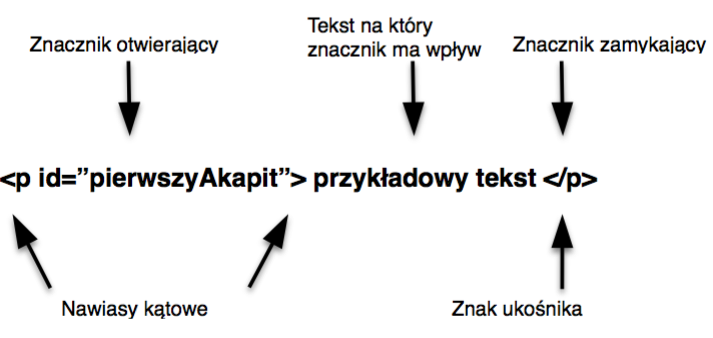
\includegraphics[scale=.5]{image/StrukturaZnacznika2.png}
\caption{Struktura znacznika}
\label{fig:Struktura znacznika}
\end{figure}
-- rysunek \ref{fig:Struktura znacznika} przedstawia strukturę elementu na przykładzie akapitu.

Atrybuty zawierają szczegółowe informacje o danych umieszczonych na stronie, natomiast same nie są tymi informacjami. Wartości atrybutów zapisywane są pomiędzy znakami apostrofu lub cudzysłowu. Prawdopodobnie najpopularniejsze są atrybuty przybierające wartości wyliczeniowe lub predefiniowane, które należą do standardowego zbioru (Listing \ref{Wartość predefiniowana})
\begin{lstlisting}[language=HTML, label=Wartość predefiniowana, caption=Wartość predefiniowana]
<link rel="stylesheet" type="text/css" 
	media="screen" href="style.css">
\end{lstlisting}
Niektóre atrybuty zapisujemy jako wartości liczbowe bądź procentowe. Przede wszystkim atrybuty, które określają wartość lub długość. Jeśli wartościom atrybutów da  się przyporządkować jakąś jednostkę, jak w przypadku wysokości tekstu lub szerokości obrazka, to zakłada się, że wartości te są wyrażone w pikselach.
Wartościami atrybutów określających kolory mogą być nazwy kolorów lub wartość zapisana szesnastkowo składająca się z koloru czerwonego, zielonego oraz niebieskiego.
Niektóre atrybuty odwołują się do innych plików i dlatego ich wartości muszą przybierać formę adresów URL (\textit{Uniform Resource Locator}) -- patrz listing \ref{Wartość predefiniowana} atrybut \textit{href} w linii numer 8.
	\begin{lstlisting}[language=HTML, label=Przykladowy HTML,  caption=Przykładowa składnia dokumentu HTML]
<!DOCTYPE html>
<html>
  <head>
   <title>Sample page</title>
  </head>
  <body>
   <h1>Sample page</h1>
   <p>This is a <a href="demo.html">simple</a> sample.</p>
   <!-- this is a comment -->
  </body>
</html>
	\end{lstlisting}
	

Każdy dokument \textit{HTML} zaczyna się deklaracją w jakim języku napisana jest strona. Przykład przedstawiony na listingu \ref{Przykladowy HTML} w linii numer 1 używa najnowszej 5 wersji specyfikacji języka \textit{HTML}. Następna część dokumentu ma charakter drzewiasty, gdzie korzeniem drzewa jest znacznik \textit{<html>} a jego potomkami \textit{<head>} oraz \textit{<body>}.

W sekcji \textit{<head>} nagłówku dokumentu określamy tytuł strony, który umieszczany jest między znacznikami \textit{<title></title>} i wyświetlany jest w pasku przeglądarki. Metadane, których zadaniem jest dostarczenie dodatkowych informacji na temat witryny i pozwalają ustalić:

\begin{itemize}
\item kodowanie znaków.
\item wskazanie języka w jakim dokument został przygotowany.
\item słowa kluczowe dla wyszukiwarki.
\end{itemize}

Znacznik \textit{<body>} odpowiada za treść, która wyświetlana jest w przeglądarce (lub innym medium, np. drukarce). Wyróżniamy trzy najważniejsze komponenty treści: zawartości tekstowej, czyli faktycznych nagłówków i akapitów, które są widoczne dla osoby przeglądającej stronę; odwołań do bardziej złożonych elementów, czyli linków, obrazków, a nawet animacji; oraz języka znaczników. Najprostszym elementem blokowym do umieszczenia zawartości tekstowej jest znacznik akapitów\textit{<p></p>}--widoczny na rysunku \ref{fig:Struktura znacznika}. Dzięki tym znacznikom przeglądarka będzie w stanie odpowiednio sformatować akapit. Znacznik akapitu może zawierać inne elementy lecz nie inne akapity. Przydatnym elementem przy formatowaniu przejścia do nowego wiersza, bez kończenia akapitu może okazać się znacznik podziału wiersza: \textit{<br />}. Aby określić unikalny identyfikator dla akapitu umieszczamy wewnątrz znacznika otwierającego atrybut \textit{id}. W przypadku gdy chcemy aby znacznik należał do grupy elementów używamy atrybutu \textit{class}. Do danej klasy może należeć dowolna ilość elementów.

Do grupowania powiązanych ze sobą obiektów służą sekcje. Pozwalają także, by grupowane wewnątrz nich obiekty korzystały ze wspólnych sposobów formatowania; wystarczy w tym celu określić sposób formatowania dla samej sekcji. Umieszczone wewnątrz sekcji obiekty dziedziczą określone cechy wyglądu, dzięki czemu nie trzeba określać formatowania osobno dla każdego z tych obiektów. 

Do budowy struktury strony wraz z wejściem standardu \textit{HTML5}, oprócz znacznika blokowego \textit{<div>}, do dyspozycji mamy elementy takie jak \textit{<section>}, \textit{<article>}, \textit{<header>} czy \textit{<footer>}. Rysunek \ref{fig:Struktura strony } przedstawia strukturę strony stworzonej przy użyciu nowych znaczników. Element \textit{<section>} reprezentuje ogólną sekcję dokumentu, bądź aplikacji. Używany jest do grupowania podobnie tematycznej treści. Za pomocą tego elementu możemy również tworzyć podsekcje, zagnieżdżając je w sobie. Przykładem takiej sekcji jest część przechowująca wpisy zamieszczone na blogu. Znacznik \textit{<article>} pozwala oznaczyć sekcję dokumentu będącą oddzielną, niezależna jego częścią. Jest wprost stworzony do opisywania właściwej treści strony internetowej. W trakcie definiowania wielu różnorodnych elementów na stronie, takich jak nagłówki, stopki, czy elementy nawigacyjne, łatwo jest zapomnieć, że najważniejsza jest treść publikowana na stronie internetowej. Treść tę opisuję właśnie znacznik \textit{<article>}. Nagłówek \textit{header}, którego nie należy mylić z nagłówkami \textit{h1, h2, h3} mogą zawierać dowolne treści od loga, a na wyszukiwarce kończąc. Na danej stronie może znajdować się jeden lub więcej nagłówków. Każda sekcja strony lub artykuł także może posiadać swój własny nagłówek, dlatego warto definiować dla każdego atrybut ID \cite{Hogan:2010:H}.
\begin{figure}[!th]
\centering
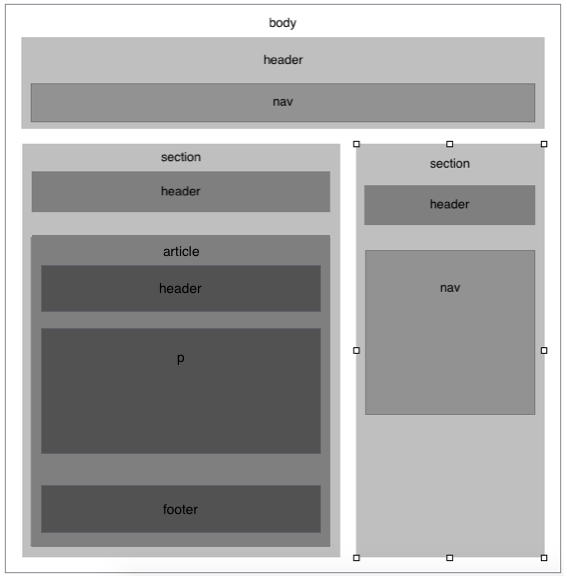
\includegraphics[scale=.6]{image/StrukturaStrony.png}
\caption{Struktura strony opisana przy użyciu nowych znaczników obecnych w HTML5}
\label{fig:Struktura strony }
\end{figure}

\subsection{CSS}

Kaskadowe arkusze stylów 	(ang. \textit{Cascading Style Sheets}, w skrócie \textit{CSS} \cite{Etemad:11:CSS}) to język używany do określenia formatowania elementów witryny internetowej, takich jak kolory, rysunki tła, czcionki, marginesy i akapity. By zwiększyć czytelność kodu \textit{HTML} i ułatwić wprowadzenie zmian do prezentacji wielu stron używających ten sam arkusz rozdzielono strukturę dokumentu od jego wyglądu. Rozdzielenie takie to również lżejsza strona, co dla  większych portali informacyjnych i użytkowników z wolniejszym łączem internetowym ma znaczenie. 

\textit{CSS} zamiast wersji posiada poziomy, każdy poziom budowany jest na podstawie poprzedniego poprzez udoskonalenia definicji i dodawania nowych funkcjonalności. Obecnie posiada trzy poziomy dwa z nich to obowiązujące specyfikacje, trzeci natomiast ma status rekomendacji. Konsorcjum \textit{W3C}  by przyśpieszyć prace nad wdrażaniem standardu \textit{CSS3} w przeglądarkach, postanowiło podzielić go na moduły. Każdy z tych modułów odpowiada za oddzielne części, takie jak transformacja 2D, tła czy obramowania. Status oficjalnego standardu na tą chwilę otrzymało tylko dwa moduły: CSS3 Colors oraz CSS3 Selectors.

\textit{CSS} by spełniał swoje zadanie, musi być przypisany do dokumentu strukturalnego. Pierwszym sposobem o najmniejszym zasięgu jest styl lokalny. Metoda ta pozwala na ustawienie wyglądu tylko dla jednego elementu, w którym zostanie osadzony. Fragment kodu w listingu \ref{Styl Lokalny} odniesie skutek tylko do nagłówka \textit{h1}.
\begin{lstlisting}[language=HTML, label=Styl Lokalny, caption=Styl lokalny]
<h1 style = "deklaracja;deklaracja;deklaracja" ></h1>
\end{lstlisting} 
Styl ten zapisuję się jako atrybut znacznika \textit{HTML}. Deklaracje wymienione są w cudzysłowie, którego pominąć nie można tak jak w przypadku innych atrybutów \textit{HTML}. Pominięcie cudzysłowia spowoduje unieważnienie stylu i nie zadziała on w żadnej przeglądarce.
Innym sposobem na umieszczenie \textit{CSS} w kodzie \textit{HTML} jest wewnętrzny arkusz stylów. Podobnie jak w przypadku stylu lokalnego ma on ograniczony zasięg, jednak reguła ta będzie się odnosić nie do jednego elementu lecz całego dokumentu. W listingu \ref{Arkusz Wewnętrzny} przedstawiony został arkusz dla wersji \textit{HTML5}.
\begin{lstlisting}[language=HTML, label=Arkusz Wewnętrzny, caption=Wewnętrzny arkusz stylów]
<head>
 <style>
  selektor { deklaracje }
 </style>
</head>
\end{lstlisting}
Najczęściej stosowanym sposobem i zarazem najlepszą metodą na zmianę wyglądu całej struktury za jednym zamachem jest dołączenie zewnętrznego arkusza stylów. Aby to zrobić w sekcji \textit{<head>} każdego dokumentu \textit{HTML} dodajemy wiersz kodu widoczny na listingu \ref{Arkusz Zewnętrzny} w linii 2.
\begin{lstlisting}[language=HTML, label=Arkusz Zewnętrzny, caption=Zewnętrzny arkusz stylów]
<head>
<link href="style.css" rel="stylesheet" >
</head>
\end{lstlisting}
Atrybut \textit{href} odpowiada za ścieżkę dostępu do zewnętrznego arkusza stylów. Drugi atrybut musi mieć wartość \textit{stylesheet} i nie możemy go pominąć. Jego brak sprawi, że arkusz nie zadziała. W \textit{HTML} nie musimy podawać atrybutu \textit{type} o wartości \textit{text/css}, bowiem dla znacznika \textit{<link>} został on ustawiony atrybutem domyślnym. Do jednego dokumentu \textit{HTML} można jednocześnie dołączyć kilka zewnętrznych arkuszy stylów, jednak najwyższy priorytet zawsze będzie miał arkusz dołączony na samym końcu. Innym ważnym atrybutem odpowiadającym za przełączanie pomiędzy alternatywnymi arkuszami jest \textit{title} a jego wartość jest jego nazwa.


Ważnym pojęciem stosowanym w kaskadowych arkuszach stylów, jest kaskadowość. Funkcja ta odpowiada za określenie hierarchii stosowanych stylów w dokumencie. Zasada kaskadowości przyjęta przez twórców polega tym, że najpierw ładowane i uwzględnianie są zewnętrzne arkusze, następnie style wpisane do nagłówka \textit{<head></head>}, a na samym końcu style wpisane bezpośrednio do znacznika. Takie rozwiązanie umożliwia pełną kontrolę nad dokumentem, a w przypadku sprzeczności zdefiniowanych stylów użyty zostanie ten, który jest najbliżej formatowanego dokumentu\footnote{\url{http://webmaster.helion.pl/index.php/pcss-dziedziczenie-i-kaskadowosc} czas dostępu: 2016-04-21}.

Za pomocą dziedziczenia polegającego na przejmowaniu przez elementy podrzędne właściwości przodków\textit{CSS} oszczędza twórcy strony wprowadzania tych samych cech dla każdego elementu z osobna. 
\begin{lstlisting}[language=HTML, label=Dziedziczenie CSS, caption=Dziedziczenie w CSS]
<!DOCTYPE html>
<html>
 <head>
  <title>Dziedziczenie w CSS</title>
  <style type="text/css">
   table {
    font-family: Verdana;
    }
   </head>
 <body>
  <table>
  <tr>
   <th>Kolumna</th>  
  </tr>
  <tr>
   <td>Komorka</td>
  </tr>  
  </table> 
 </body>
</html>
\end{lstlisting} 
Widoczny na listingu \ref{Dziedziczenie CSS} przykład przedstawia dziedziczenie przez elementy potomne \textit{<tr>}, \textit{<th>} i \textit{<td>}, właściwości \textit{font-family}. Ciało dokumentu\textit{<body>} (element nadrzędny) nie dziedziczy czcionki, bowiem jest przodkiem tabeli, a nie jej potomkiem. Jednak nie wszystkie cechy przekazywane są z pokolenia na pokolenia. Marginesy i dopełnienia są przykładami cech, będącymi wyjątkiem od tej reguły. Jednak jeśli jakaś cecha nie jest dziedziczona, dzięki \textit{inherit} jesteśmy w stanie wymusić nadanie tej właściwości. 

Podstawowa konstrukcja stylu \textit{CSS} posiada selektor oraz deklaracje stylu. Selektor jest elementem \textit{HTML} do którego będą stosowane deklaracje. Deklaracja stylu umieszczana jest zawsze w nawiasie klamrowym i określa właściwości umożliwiające modyfikację wglądu lub zachowania elementu. Najprostszym selektorem jest zwykły selektor elementu przedstawiony na listingu \ref{Selektor}. Przypisanie znacznikowi \textit{p} właściwości \textit{color: red;} spowoduję, że wszystkie elementy o tej samej nazwie zostaną sformatowane zgodnie z definicją.
\begin{lstlisting}[label=Selektor, caption=Selektor elementu,float=ht]
 p{ 
   color:red;
 }
\end{lstlisting}
Selektor uniwersalny widoczny na listingu \ref{Selektor Uniwersalny}, przypisuję właściwość \textit{color: green;} do wszystkich elementów języka \textit{HTML}. 
\begin{lstlisting}[label=Selektor Uniwersalny, caption=Selektor uniwersalny]
*{
 color: green;
 }
\end{lstlisting}
Selektor klasy pozwala nam nadać identyczne formatowanie pogrupowanym przez nas elementom. Listing  \ref{Selektor Klasy} przedstawia dwie zasady dotyczące klas, pierwsza z nich mówi, że ta sama klasa może być użyta w wielu elementach oraz więcej niż jedna klasa może opisywać element.
\begin{lstlisting}[label=Selektor Klasy, caption=Selektor klasy]
p.klasa1{
 font-size: 10px;
}

h1.klasa2{
color: yellow;
}

<p class="klasa1">tekst akapitu</p>
<h1 class="klasa1 klasa2">tekst naglowka</p>
\end{lstlisting}
 Selektorem pozwalającym odniesienie się do konkretnego elementu bez naruszenie pozostałych jest identyfikator widoczny na listingu \ref{Selektor identyfikator}. Możemy go nadać dla dowolnego elementu języka \textit{HTML}. W przeciwieństwie do klas, każdy element może mieć tylko jeden identyfikator, który jest unikalnym atrybutem i może wystąpić tylko raz w danym dokumencie. 
 \begin{lstlisting}[label=Selektor identyfikator, caption=Selektor identyfikatora]
#identyfikator {
 font-size: 50px;
 }
 
 <p id="identyfikator">tekst akapitu</p>
 \end{lstlisting}
\subsection{JavaScript}

\textit{JavaScript} to język programowania pozwalający stworzyć program, który może być włączony do strony \textit{HTML}. Zamknięty jest w znacznikach \textit{<script>}, dlatego jego tekst nie pojawia się na ekranie, a przeglądarka ,,wie'', że zamiast wyświetlać tekst skryptu, ma go wykonać. Znacznik \textit{<script>} najczęściej można znaleźć w sekcji \textit{<head>} strony \textit{HTML}, chociaż skrypty można też umieszczać w sekcji \textit{<body>}. W tym miejscu najlepiej umieszczać skrypty, które wypisują tekst na ekranie lub tworzą kod \textit{HTML} \cite{Negrino:2007:J}.

Język \textit{JavaScript} został opracowany przez \textit{Netscape Communications Corporation} -- firmę, która stworzyła przeglądarkę \textit{WWW}. \textit{JavaScript} był pierwszym językiem skryptowym obsługiwanym przez przeglądarki i nadal pozostaje zdecydowanie najpopularniejszym z nich. Według ECMA -- która standaryzuje ECMAScript, podzbiór JavaScriptu -- językiem skryptowym nazywamy język programowania stworzony do manipulowania, dostosowywania i automatyzowania obiektów istniejącego już systemu. Poprzez interfejs użytkownika w systemie dostępna jest użyteczna funkcjonalność a język skryptowy jest mechanizmem, który uwidacznia tą funkcjonalność programując kontrole. Tym sposobem komunikujemy istniejącemu systemowi by zapewnił środowisko obiektów i udogodnień co uzupełnia możliwości języka skryptowego.

Dzięki językowi \textit{JavaScript} jesteśmy w stanie wyświetlać wszelkiego rodzaju komunikaty dla użytkownika w obrębie strony \textit{WWW}, jak i na pasku stanu przeglądarki oraz w ramkach ostrzegawczych. Kontrolować czy użytkownik poprawnie wypełnia dane formularza lub przeprowadzać obliczenia. Tworzyć paski reklamowe pozwalające na interakcje z użytkownikiem zamiast wyświetlanie zwykłych obrazków. Wykrywać typy przeglądarek oraz wykonywać zaawansowane funkcje w tylko tych przeglądarkach, które je obsługują. Sprawdzać zainstalowane moduły dodatkowe i powiadamiać użytkownika, gdy jest potrzeba zainstalowania dodatkowego modułu. Użytkownik nie jest zmuszany do przeładowania strony gdy modyfikujemy jej część.

 \begin{lstlisting}[label=Skrypt w JavaScript, caption=Skrypt w JavaScript]
<html>
 <head>
  <title>Data i godzina</title>
  <meta http-equiv="Content-Type" content="text/html">  
 </head>
 <body>
  <h1>Data i czas</h1>
  <p>
   <script language="JavaScript" type="text/javascript">
   var teraz = new Date();
   var czasLokalny = teraz.toString();
   document.write("<b>Czas lokalny:</b>" + czasLokalny);
   </script> 
  </p> 
 </body>
</html>
 \end{lstlisting}

Widoczny na listingu \ref{Skrypt w JavaScript} przykładowy skrypt umieszczony w znaczniku \textit{HTML} wyświetli bieżący czas w przeglądarce użytkownika. Za pomocą instrukcji \textit{teraz = new Date();} do zmiennej \textit{teraz} przypiszemy obiekt typu \textit{Date()}. Zmienne w \textit{JavaScripcie} są kontenerami, które przechowują różnego typu dane (np. liczbę, łańcuch tekstu lub obiekt). Nazwa zmiennej może zawierać litery duże jak i małe alfabetu oraz cyfry od 0 do 9. Istnieją dwa typy zmiennych: globalna i lokalna. Zmienna globalna, która ma zasięg we wszystkich skryptach dokumentu \textit{HTML}, powinna być zadeklarowana w głównym skrypcie, na zewnątrz wszelkich funkcji. Natomiast zmienna lokalna może być używana tylko w funkcji, w której została utworzona. Metoda \textit{toString()} obiektu \textit{teraz} skonwertowała datę do zmiennej typu \textit{String}, dzięki czemu funkcja \textit{document.write()} wyświetliła aktualny czas użytkownika.

Komentarze w JavaScript umożliwiają umieszczenie dokumentacji kodu  wew\-nątrz skryptu. Pozwala to innym zrozumieć działanie skryptu lub zapobiega egzekucji kodu gdy testujemy alternatywne rozwiązania. Aby zawrzeć komentarz w programie JavaScript do wyboru mamy dwa typy komentarzy. Liniowy -- widoczny na listingu \ref{Komentarz w JavaScript} -- zaczyna się od dwóch ukośników a kończy przy przejściu do następnej linii. Drugim typem komentarzy obsługiwanym przez JavaScript jest  styl języka C, nazywany blokowym. Rozpoczyna się od sekwencji znaków \textit{/*} a kończy tymi samymi znakami tylko w odwrotnej kolejności. Komentarze takie mogą zawierać więcej niż jeden wiersz kodu, jak w listingu \ref{Komentarz w JavaScript} wierszu 2 i 3. Instrukcje JavaScript w komentarzu są ignorowane więc przy usuwaniu błędów w skrypcie gdy potrzebujemy chwilowo wyłączyć część sekcji programu możemy dodać \textit{/*} na początku i \textit{*/} na końcu komentując fragment kodu.
\begin{lstlisting}[label=Komentarz w JavaScript, caption=Komentarz liniowy i blokowy]
//Komentarz liniowy
/*Komentarz blokowy wiersz pierwszy
Komentarz blokowy wiersz drugi*/
\end{lstlisting}
\section{Biblioteki języka JavaScript}
Biblioteki \textit{JavaScript} to fragmenty kodu napisanego w tym języku, które zawierają rozwiązania wielu prozaicznych zadań wykonywanych każdego dnia przez programistów. Można je sobie wyobrazić jako kolekcje gotowych funkcji \textit{JavaScriptu}, które wystarczy dodać do strony. Funkcje te ułatwiają wykonywanie najczęściej spotykanych zadań. Często zdarza się, że bardzo wiele wierszy naszego własnego kodu (oraz sporo godzin koniecznych do jego napisania) można zastąpić wywołaniem jednej funkcji takiej biblioteki. Istnieje bardzo dużo takich bibliotek, a wielu z nich używano podczas tworzenia największych i najbardziej znanych stron \textit{WWW}, takich jak Yahoo, Amazon, CNN, Apple oraz Twitter \cite{McFarland:2012:JS}. Kilka najbardziej znanych bibliotek:
\begin{itemize}
\item Yahoo User Interface Library (\textit{http://developer.yahoo.com/yui/}) -- projekt stworzony i używany przez Yahoo. Twórcy rozwijają i poprawiają tą biblioteka, posiada także dobrą dokumentacje.
\item Dojo Toolkit (\textit{http://dojotoolkit.org/}) -- kolekcja bardzo wielu plików \textit{JavaScript} mogących rozwiązać nurtujący nas problem związany z tworzeniem skryptów.
\item Mootools (\textit{/http://mootools.net/}) -- biblioteka pomagająca tworzyć płynne animacje i innych efektów wizualnych.
\item Prototype (\textit{http://www.prototypejs.org/}) -- jedna z pierwszych bibliotek \textit{JavaScript} jaka się pojawiła. Zawiera przydatne rozszerzenia do środowiska skryptowego przeglądarki oraz zapewnia eleganckie \textit{API} dla interfejsu \textit{Ajax}.
\end{itemize}
\subsection{jQuery}
jQuery jest biblioteką języka \textit{JavaScript}, która przyśpiesza i ułatwia programowanie ponieważ samoczynnie wykonuję złożone zadania. Pozwala łatwo manipulować stroną \textit{HTML}	po jej wyświetleniu przez przeglądarkę. Dostarcza narzędzi, które pomagają nam nasłuchiwać co użytkownik wykonuję na stronie, do tworzenia animacji, oraz funkcje pozwalające komunikowanie się z serwerem bez przeładowywania strony. 

Podobnie jak w przypadku zewnętrznych plików \textit{JavaScript} skrypty \textit{jQuery}, by zaczęły działać muszą być dołączone do swojej strony. Istnieje kilka sposobów pozwalające nam to zrobić: można pobrać bibliotekę udostępnioną przez \textit{Google}, \textit{Microsoft} lub \textit{jQuery.com} albo skopiować plik biblioteki na własny komputer i umieścić go na stronie.
Korzystając z sieci dystrybucji treści (ang. \textit{content distribution network}) -- innej strony przechowującej i udostępniającej bibliotekę--obniżamy obciążenie własnego serwera, ponieważ to serwery \textit{Google} czy \textit{Microsoftu} użyczają bibliotekę użytkownikom przeglądającym witrynę. Inną korzyścią tego rozwiązania jest, że serwery tych firm rozmieszczone są na całym świecie, więc osoba przeglądająca stronę pobierze plik biblioteki z serwera położonego znacznie bliżej swojego miejsca zamieszkania niż nasz, co przyspieszy transfer i nasza witryna szybciej zadziała. Takie rozwiązanie ma też ważną wadę, użytkownik przeglądający naszą witrynę musi być podłączony do internetu by ściągnąć plik pozwalający poprawne działanie strony. Listing  \ref{CDN Google} przedstawia pobranie biblioteki z serwera Google.

\begin{lstlisting}[label=CDN Google, caption=Pobranie biblioteki z serwera Google]
<script src="https://ajax.googleapis.com/ajax/libs/jquery/2.1.3/jquery.min.js"></script>
\end{lstlisting}

Drugim sposobem dodania biblioteki \textit{jQuery} jest pobranie i umieszczenie pliku na stronie. Plik ten jest zewnętrznym plikiem \textit{JavaScriptu} i dodaje się go do strony poprzez komendę widoczną na listingu \ref{Zewnetrzny plik}.
\begin{lstlisting}[label=Zewnetrzny plik, caption=Dodanie zewnętrznego pliku jQuery]
<script src="jquery-2.1.3.min.js"></script>
\end{lstlisting}

Funkcje są potrzebnym narzędziem, dzięki którym w wydajny sposób możemy wielokrotnie powtarzać te same operacje. W \textit{jQuery} funkcje mogą być zapisywane w skrócie jako \textit{\$()} i wykorzystywane na jeden z czterech sposobów. Pierwszy sposób -- widoczny na listingu \ref{Parametr funkcja} -- jako pierwszy parametr przyjmuje inną funkcje o nazwie \textit{powitanieAplikacji()} w wierszu 11.

\begin{lstlisting}[label=Parametr funkcja, caption=Wywołanie funkcji przyjmującej inną funkcje jako parametr]
<!DOCTYPE html>
<html>
 <head>
  <title>Funkcja jako parametr</title>
  <script type="text/javascript" src="jquery-2.1.3.min.js"></script>
  <script type="text/javascript">
   function powitanieAplikacji()
   {
   	alert('Hello');
   }
   $(powitanieAplikacji);
  </script>
 </head>
 <body>
  ...
  </body>
</html>
\end{lstlisting}

Drugim sposobem wywołania funkcji \textit{jQuery} -- pokazany na listingu \ref{Parametr kod XHTML} -- jest przekazanie kodu XHTML jako pierwszego parametru. W wierszu 8 utworzyliśmy nowy węzeł DOM (ang. \textit{Document Object Model}) i dowiązaliśmy go do bieżącego dokumentu wywołując metodę \textit{.appendTo()}. Należy pamiętać by instrukcja widoczna w wierszu 8 była zapisana w jednym wierszu, ponieważ napisy w języku \textit{JavaScript} nie mogą wydłużać się na wiele wierszy. Gdy napis rozciągnie się na więcej niż jeden wiersz otrzymamy błędy kod \textit{JavaScriptu}.

\begin{lstlisting}[label=Parametr kod XHTML, caption=Wywołanie funkcji przyjmującej jako pierwszy parametr kod XHTML]
<!DOCTYPE html>
<html>
 <head>
  <title>Kod XHTML jako parametr</title>
  <script type="text/javascript" src="jquery-2.1.3.min.js"></script>
  <script type="text/javascript">
  $(function(){
  	$('<div id="nowyElement"><p>Hello</p></div>').appendTo('body');  
  });  
  </script>
 </head>
 <body>
  ...
  </body>
</html>
\end{lstlisting} 

Trzecim sposobem przedstawionym na listingu \ref{Parametr selektor} jest wywołanie funkcji z selektorem jako pierwszym parametrem. W wierszu 10 wywołanie przyjmuję jeszcze jeden opcjonalny parametr, nazywany \textit{kontekstem}. Kontekst jest obiektem \textit{DOM} lub \textit{jQuery}, ograniczający zasięg selektora. Kod w wierszu 8 i 9 utworzy zmienną \textit{g}, która będzie obiektem \textit{jQuery} zawierający identyfikator \textit{\#gora}.

\begin{lstlisting}[label=Parametr selektor, caption=Wywołanie funkcji przyjmującej jako parametr selektor]
<!DOCTYPE html>
<html>
 <head>
  <title>Selektor jako parametr</title>
  <script type="text/javascript" src="jquery-2.1.3.min.js"></script>
  <script type="text/javascript">
  $(function(){
  var g = $('#gora');
  $('h1' , g).css('color' , 'green');
  }):
  </head>
  <body>
   <div>
    <h1>Naglowek</h1>
   </div>
   <div id="gora">
   <h1>Naglowek2</h1>   
   </div>
  </body>
 </html>
\end{lstlisting}

Kolejnym sposobem wywołania funkcji \textit{\$()}, jest przyjęcie jako pierwszy parametr element drzewa \textit{DOM} lub tablice takich elementów. Widoczna na listingu \ref{Parametr element DOM} w wierszu 8 i 9, zmienna \textit{element} przyjmuję wynik działania metody \textit{getElementById()} i wywołana zostaje funkcja z tym elementem drzewa \textit{DOM}.

\begin{lstlisting}[label=Parametr element DOM, caption=Wywołanie funkcji przyjmującej jako parametr element drzewa DOM]
<!DOCTYPE html>
<html>
 <head>
  <title>Element DOM jako parametr</title>
  <script type="text/javascript" src="jquery-2.1.3.min.js"></script>
  <script type="text/javascript">
  $(function(){
  var element = document.getElementById('gora');
  $(element).text('...');
    }):
  </head>
  <body>
   <div id="gora">
   </div>
 </body>
</html>
\end{lstlisting}

\subsection{jQuery Mobile}
\textit{jQuery Mobile} jest zbiorem wtyczek i kontrolek mających na celu tworzenie mobilnych aplikacji internetowych na różne platformy. W odniesieniu do implementacji kodu, \textit{jQuery Mobile} przypomina bardzo bibliotekę \textit{jQuery UI}, z tym że \textit{jQuery UI} skoncentrowana jest na tworzenie aplikacji desktopowych, zaś \textit{jQuery Mobile} przeznaczona jest do aplikacji mobilnych. W bibliotece tej aby uzyskać konsekwentny efekt dla różnych platform mobilnych użyto atrybutów \textit{HTML5} i właściwości \textit{CSS3} by wzbogacić podstawowe znaczniki \textit{HTML}. Dzięki skorzystaniu ze specyfikacji \textit{HTML5} w zakresie spersonalizowanych atrybutów obsługi danych możliwe jest osadzenie danych w kodzie znaczników \textit{HTML5}. Po załadowaniu biblioteki \textit{jQuery Mobile} wybiera ona elementy na postawie ich atrybutów obsługi danych, po czym poprawia je poprzez wprowadzenie nowych znaczników, dodanie procedur obsługi zdarzeń, oraz stworzenie nowych klas \textit{CSS}. Dzięki temu można szybko stworzyć podstawowy kod złożony z podstawowych znaczników, a \textit{jQueryMobile} przekształci to na złożone elementy interfejsu użytkownika. 

Widoczna na listingu \ref{Strona jQueryMobile} podstawowa struktura strony korzystająca z biblioteki \textit{jQuery Mobile} jest przygotowana w specyficzny sposób. 

\begin{lstlisting}[label=Strona jQueryMobile, caption=Prosta strona HTML5 dla aplikacji jQuery Mobile]
<!DOCTYPE html> 
<html>
 <head>
 <title>Podstawowa strona</title>
 <meta name="viewport" content="width=device-width, initial-scale=1">
 <link rel="stylesheet" href= "http://code.jquery.com/mobile/1.4.5/jquery.mobile-1.4.5.min.css">
 <script type="http://code.jquery.com/jquery-1.11.1.min.js"> </script>
 <script type="http://code.jquery.com/mobile/1.4.5/jquery.mobile-1.4.5.min.css"> </script>
 </head> 
 <body>
 <div data-role="page">
  <div data-role="header"> <h2>Tytul strony</h2>
 </div>
 <div data-role="content"> <p>Hello world!</p>
 </div> 
 </div>
 </body> 
</html>
\end{lstlisting}
W wierszu 4 jest znacznik \textit{viewport}, który prosi urządzenie w ustawienie określonego poziomu powiększenia oraz wielkość strony i dopasowanie ich do aktualnie wyświetlanej zawartości. Ma to kluczowe znaczenie przy tworzeniu witryn przeznaczonych dla urządzeń mobilnych. Domyślna wartość tego znacznika jest zależna od przeglądarki ale przeważnie wynosi około 980 pikseli. W przypadku większej lub mniejszej rozdzielczości urządzenia od domyślnej, układ strony może wydawać się zbyt mały lub powiększenie zostanie ustawione w taki sposób, że tekst będzie zbyt mały do wygodnego czytania. Dzięki określeniu atrybutów \textit{width} oraz \textit{initial--scale} rozmiar ekranu urządzenia możemy dostosować do wielkości zawartości. 

Określamy używany arkusz stylów \textit{CSS} za pomocą instrukcji widocznej w wierszu 6. Przy jego użyciu można zmienić całkowity wygląd strony. Trzeba jednak wziąć pod uwagę liczbę urządzeń, na jakich witryna zostanie przetestowana. Domyślnie biblioteka \textit{jQuery Mobile} testowana jest na dużej liczbie urządzeń.

W wierszach 8 i 7 znajdują się znaczniki pobierające biblioteki \textit{jQuery Core} oraz \textit{jQuery Mobile}. Sama zawartość strony umieszczona została  w wierszach 11--16. W większości jest to zwyczajny kod \textit{HTML}. Jednak każdy znacznik \textit{div} zawiera atrybut \textit{data-role} z przypisaną wartością: \textit{page}, \textit{header}, \textit{content}. Biblioteka \textit{jQuery Mobile} przypisuje za pomocą tych znaczników o określonych rolach, poszczególnym elementom witryny pasujący styl, temat czy działanie.

Biblioteka \textit{jQuery Mobile} dzięki atrybutowi \textit{data-role} oznacza strony oraz elementy na podstawie ich atrybutów, po czym ulepsza  wprowadzając klasy \textit{CSS}, potrzebne znaczniki oraz obsługę zdarzeń. Stosowanie takiej metody przez \textit{jQuery Mobile} prowadzi do płynnych przejść między stronami, automatycznego obsługiwania nawigacji oraz lepszej wydajności ponieważ zasoby zapisane są w jednym pliku. 
Na listingu \ref{Strony wewnętrzne} przedstawiona została metoda, która za pomocą atrybutu \textit{data-role="page"} widocznego w wierszu 12 i 21 oznaczyła oddzielne sekcje treści jako strony. Nie jest możliwe zagnieżdżanie stron wewnątrz siebie, sekcje odpowiadające za strony muszą być rodzeństwem najwyższego poziomu drzewa dokumentu.

Biblioteka \textit{jQuery Mobile} jest w stanie zarządzać także stronami zewnętrznymi. Gdy łącze zostanie zdefiniowane do osobnej strony zamiast do ID elementu \textit{data-role="page"} będącego w bieżącym dokumencie \textit{jQuery Mobile} asynchronicznie pobiera żądaną stronę. Następnie przeszukuję ją w by znaleźć pierwszy element oznaczony atrybutem \textit{data-role="page"} i wstawia go do dokumentu źródłowego. Reszta treści, razem z kolejnymi elementami z atrybutami \textit{data-role="page"} jest ignorowana. Gdyby ściąganie strony zakończyło się niepomyślnie lub \textit{jQuery Mobile} nie znajdzie elementu oznaczonego szukanym atrybutem, wyświetli komunikat o błędzie. 

W przypadku gdy chcemy załadować stronę rezygnując by biblioteka \textit{jQuery Mobile} pobrała ją asynchronicznie i scaliła z bieżącym modelem DOM możemy załadować stronę z wykorzystaniem technologii \textit{AJAX} określając atrybut \textit{target} łącza (na przykład na "blank") lub ustawiając atrybut \textit{rel=''externa''}\cite{Holzner:2008:AJAX}.
\clearpage
\begin{lstlisting}[label=Strony wewnętrzne, caption=W pojedynczym dokumencie HTML zawarte są dwie wewnętrzne strony]
<!DOCTYPE html> 
<html>
 <head>
 <title>Strony wewnetrzne</title>
 <meta name="viewport" content="width=device-width, initial-scale=1">
 <link rel="stylesheet" href= "http://code.jquery.com/mobile/1.4.5/jquery.mobile-1.4.5.min.css">
 <script type="http://code.jquery.com/jquery-1.11.1.min.js"> </script>
 <script type="http://code.jquery.com/mobile/1.4.5/jquery.mobile-1.4.5.min.css"> </script>
 </head> 
 <body>
 <!--Strona pierwsza-->
<section id="strona1" data-role="page">
<header data-role="header"><h1>Przyklad strony</h1></header> 
<div data-role="content" class="content">
<p>Strona Pierwsza</p>
<p><a href="#strona2">Przejscie do strony drugiej</a></p> 
</div>
</section>

<!--Strona druga-->
<section id="strona2" data-role="page">
<header data-role="header"><h1>Przyklad stron wewnetrznych</h1></header> 
<div data-role="content" class="content">
<p>Strona druga</p>
<p><a href="#strona1">Przejscie spowrotem do strony pierwszej</a></p> 
</div>
</section>
 </body> 
</html>
\end{lstlisting}
\section{Reprezentacja danych}
Wraz z rozpowszechnieniem internetu oraz jego zasobów informacyjnych w postaci stron \textit{WWW}, pojawił się pomysł do wykorzystania ich jako baz danych. Jednak dane przechowywane w postaci stron \textit{HTML} w przeciwieństwie do relacyjnych baz danych nie mają tak regularnej struktury. Do opisanie takich danych używa się określenia dane semistrukturalne -- czyli model danych różniący się od formalnej struktury danych powiązanych z relacyjnymi bazami danych ale zawierający tagi pozwalające rozdzielić oraz wymusić hierarchie rekordów. Podstawą matematyczną takiego modelu jest graf skierowany, co czynni reprezentacje danych na bardziej elastyczną niż w relacyjnych bazach danych. W semistrukturalnych danych wpisy należące to tej samej klasy mogą posiadać różne atrybuty nawet gdy są pogrupowane razem oraz kolejność atrybutów nie jest istotna. 
\subsection{JSON}
\textit{JSON} (ang. \textit{Java Script Object Notation}) \cite{Bray:05:JSON} czyli prosty format wymiany danych oparty na języku programowania \textit{JavaScript}. Choć jest całkowicie niezależny od innych języków programowania jest formatem tekstowym używającym zwyczajów praktyk z innych języków jak \textit{C}, \textit{C++}, \textit{Java}, \textit{Perl} czy \textit{Python}. \textit{JSON} ukształtował się na bazie dwóch charakteryzujących go struktur. Pierwszą z nich jest zbiór par nazwa i wartość. W innych językach może występować jako rekord, struktura czy tabela asocjacyjna. Drugą strukturą jest uporządkowana lista wartości. Implementowana za pomocą tabeli czy listy w innych językach.
Większość nowoczesnych języków programowania używa tych uniwersalnych struktur danych, dlatego też format danych opiera swoją budowę na przytoczonych strukturach. 

\begin{lstlisting}[label=Struktura danych JSON, caption=Przykładowa struktura danych w formacie JSON]
{
 "uczelnia": {
 	"wyklad": {
 		"typ": "seminarium",
 		"wyklad_tytul": "Podstawy JSON",
 		"wyklad_numer": "9.10",
 		"data_rozpoczecia": "12-12-2015",
 		"studenci": {
 			"student": [
 			{
 			"status":"obecny",
 			"imie": "Edward",
 			"nazwisko": "Nozycoreki"
 			},
 			{
 			"status":"nieobecny",
 			"imie": "Leon",
 			"nazwisko": "Zawodowiec"
 			}
 			]}
 	}
}
 			
\end{lstlisting}
\subsection{XML}
\textit{XML} (ang. \textit{Extensible Markup Language}) \cite{Bray:11:XML} jest rozszerzalnym językiem znaczników opartym na \textit{Standardowym uogólnionym językiem znaczników} (SGML). Jak sama nazwa wskazuję \textit{SGML} jest językiem bardzo ogólnym o ogromnych możliwościach, niestety ceną za te możliwości jest złożoność, co utrudnia jego naukę. \textit{XML} służy do definiowania pozostałych języków zwany metajęzykiem. W przeciwieństwie jednak to swego przodka jest prostszy i bardziej praktyczny. W języku tym nie sprecyzowano ani zestawu znaczników, a gramatyki. Zestaw znaczników określa jakie znaczniki są ważne dla parsera znaczników. \textit{XML} nie ma zdefiniowanego ani zestawu znaczników, ani gramatyki. Posiada więc nieograniczone możliwości rozbudowy. Choć elastyczność jest jedną największych zalet \textit{XML}, to jest też jednak jedną z jego wad. Dokumenty \textit{XML} możemy przedstawiać na tyle różnych sposobów, że powstała bardzo duża liczba standardów opisujących tłumaczenia formatów danych i same formaty.

\textit{XML} pozwala także określić strukturę i sposób umieszczenia jednych elementów w innych. 
Listing \ref{Dokument XML} przedstawia dokument \textit{XML} opisujący seminarium oraz obecność dwóch studentów. W dokumencie takim możemy wymusić by każdy element \textit{<student>} zawierał dokładnie po jednym elemencie \textit{<imie>} i \textit{<nazwisko>} lub nie zawierał elementu \textit{<wyklad\_numer>}.
\begin{lstlisting}[label=Dokument XML, caption=Przykładowy dokument XML]
<?xml version="1.0" encoding="UTF-8">
<uczelnia>
 <wyklad typ="seminarium">
  <wyklad_tytul>Podstawy XML</wyklad_tytul>	
  <wyklad_numer>9.10</wyklad_numer>
  <data_rozpoczenia>12-12-2015</data_rozpoczenia>
  <studenci>
   <student status="obecny">
    <imie>Edward</imie>
    <nazwisko>Nozycoreki</nazwisko>
    </STUDENT>
   <STUDENT status="nieobecny">
    <imie>Leon</imie>
    <nazwisko>Zawodowiec</nazwisko>
   </student>
  </studenci>
 </wyklad>
</uczelnia>
\end{lstlisting}

Aby przeglądarka uznała dokument \textit{XML} przeprowadza dwie kontrole. Pierwsza polega na sprawdzeniu czy dokument jest poprawnie sformułowany czyli spełnia ustawione przez \textit{W3C} specyfikację \textit{XML} 1.0 dotyczącej składni. Oznacza to istnienie przynajmniej jednego elementu w dokumencie oraz wystąpienie elementu głównego, który zawiera wszystkie inne elementy występujące w dokumencie. Każdy element musi koniecznie być zamknięty całkowicie w elementach nadrzędnych względem niego. Przykład na listingu  \ref{Niepoprawny XML} przedstawia niepoprawnie sformułowany dokument ponieważ widoczny w wierszu 6 znacznik końcowy \textit{</naglowek>} występuje po znaczniku otwierającym następnego elementu \textit{<temat>}.
\begin{lstlisting}[label=Niepoprawny XML, caption=Niepoprawnie sformułowany dokument XML]
<?xml version="1.0" encoding="UTF-8">
<dokument>
 <naglowek>
  Hello
 <temat>
 </naglowek>
  Zle ustawione znaczniki
  </temat>
</dokument>
\end{lstlisting}

Druga kontrola przeprowadzana przez przeglądarkę jest walidacja dokumentu, która jest opcjonalna \textit{XML}. Dokument \textit{XML} można walidować, gdy definicja typu dokumentu jest z nim związana i dokument jest z nią zgodny. Definicja typu dokumentu (\textit{DTD}) ustala jego prawidłową składnię. \textit{DTD} można przechowywać na dwa sposoby: w osobnym pliku lub w tym samym dokumencie jak przestawia listing \ref{Walidacja XML}. 

\begin{lstlisting}[label=Walidacja XML, caption=Definicja typu dokumenty umieszczona w tym samym dokumencie]
<?xml version="1.0" encoding="UTF-8">
<?xml-stylesheet type="text/css" href="first.css"?>
<!DOCTYPE DOKUMENT [
	<!ELEMENT DOKUMENT (NAGLOWEK, TEMAT)>
	<!ELEMENT NAGLOWEK (#PCDATA)>
	<!ELEMENT TEMAT (#PCDATA)>
	]>
<dokument>
 <naglowek>
  Hello
 <temat>
 </naglowek>
  Zle ustawione znaczniki
  </temat>
</dokument>
\end{lstlisting}
\subsection{Atom}
\textit{Atom} \cite{Nottingam:05:Atom} jest formatem dokumentu opartym na \textit{XML}, który opisuje listę powiązanych ze sobą informacji znanych jako kanał.  \textit{Kanały} są zbudowane z pewnej liczby elementów przedstawionych jako \textit{wpisy}, każdy \textit{wpis} zawiera rozszerzalny zestaw dołączonych metadanych. Dla przykładu w przedstawionym listingu \ref{Przyklad Kanalu} \textbf{wpis} posiada metadane \textit{<title></title>} w wierszu 13.
Standard \textit{Atom} stworzony został z myślą rozwiązania problemu z błędami specyfikacji równoległych standardów \textit{RSS}. Unika on niejasności wyżej wymienionej specyfikacji, poprawia zgodność z \textit{XML} i innym standardami oraz określa protokół publikacji kanałów.
\begin{lstlisting}[label=Przyklad Kanalu, caption=Przykład wpisu w Atom]

 <?xml version="1.0" encoding="utf-8"?>
   <feed xmlns="http://www.w3.org/2005/Atom">
	<link href="http://www.example.com" rel="alternate" type="text/html" />
	<updated>2016-01-11T18:30:02Z</updated>
     <title>Przyklad wpisu</title>
     <author>
       <name>Jan Kowalski </name>
     </author>
     <id>urn:uuid:60a76c80-d399-11d9-b93C-0003939e0af6</id>

     <entry>
       <title>Przykladowy tytul hasla</title>
       <link href="http://example.org/2003/12/13/atom03"/>
       <id>urn:uuid:1225c695-cfb8-4ebb-aaaa-80da344efa6a</id>
       <updated>2016-01-13T18:30:02Z</updated>
       <summary>Jakis tekst.</summary>
     </entry>

   </feed>

\end{lstlisting}

Wiele z elementów \textit{Atom} posiadają kilka podobnych struktur, takie jak struktura tekstu, daty czy osoby. Kiedy element jest zdefiniowany jako określona typ struktury, dziedziczy on wyszczególnione wymogi z definicji struktury tej sekcji. Struktura tekstu \textit{Atom} zawiera zazwyczaj małej zawartości tekst czytelny dla człowieka. Przedstawiona na listingu \ref{Struktura tekstu} struktura zawiera atrybut \textit{type} w wierszu 4 oznacza to, że wartość tej struktury musi być typu "text" lub "html". Jeżeli nie zdefiniujemy tego atrybutu, \textit{Atom}  domyślnie będzie się zachowywał jakby atrybut ten był ustawiony na "text".

\begin{lstlisting}[label=Struktura tekstu, caption=Struktura tekstu w Atom]

 atomPlainTextConstruct =
      atomCommonAttributes,
      attribute type { "text" | "html" }?,
      text
   
\end{lstlisting}

Struktura osoby jest elementem opisującym osobę, korporację lub inne podobne hasło. W specyfikacji tej kolejność pojawiania się elementów pochodnych nie ma znaczenia. Element \textit{name} jako wartość przyjmuje czytelną dla człowieka nazwę oraz opisana osoba może posiadać tylko jeden taki element. Ta sama reguła obowiązuję dla pozostałych elementów \textit{uri} oraz \textit{email}, z wyjątkiem, tego że \textit{uri} zawiera adres \textit{IRI} do tej osoby a element \textit{email} jego adres e-mail.

Struktura daty odpowiada za przedstawienie daty zgodnej ze standardem internetowym. W dodatku wielka litera ''T'' musi być użyta w celu oddzielenia daty od czasu, oraz litera ''Z'' gdy nie podamy numerycznie strefy czasowej. Powinna być także dokładna jak to tylko możliwe, czyli w złym zwyczaju było by ustawienie dla systemu publikacji zastosować takie same znaczniki czasu określające kilka wpisów, które miały miejsce tego samego dnia.

------%Rozdział Drugi-----

\cleardoublepage
\chapter{Platforma iOS}
\label{cha:Platforma iOS}

\section{Mobilny system operacyjny}
Mobilny system operacyjny jest oprogramowaniem pozwalającym innym programom zwanym aplikacjami uruchamiać się na urządzeniach przenośnych takich jak telefony komórkowe, smartfony czy tablety. Przez ostatnie lata projekt mobilnych systemów operacyjnych przeszedł trzy fazową ewolucję:  z systemu opartego na komputerach PC do systemów komputerowych specjalnego przeznaczenia, aby zakończyć na obecnie  obowiązującym systemie zorientowanym na smartfony. W całym procesie przemiany zmiany nastąpiły także w architekturze mobilnych systemów ze skomplikowanej przez mniej złożoną do czegoś pośrodku. Naturalnie cały proces ewolucyjny napędzany jest przez postęp technologiczny w trzech dziedzinach. Sprzęcie komputerowym, gdzie przemysł zmniejszył rozmiar mikroprocesorów i urządzeń peryferyjnych pozwalający na stworzenie dzisiejszych urządzeń mobilnych. Przed tymi zmianami nie było możliwe osiągnięcie tak wysokiej wydajności przy tak małych gabarytach. Drugą dziedziną jest oprogramowanie, które w komputerach przenośnych jest skoncentrowane na produktywności użytkownika, dlatego też wsparcie dla myszki i klawiatury było sprawą kluczową. Oprogramowanie na urządzenia mobilne pozwalały jedynie na zarządzanie kontaktami, wysyłanie wiadomości tekstowych itd. Przy czym korzystanie z tych niewielu funkcjonalności bez obsługi ekranu dotykowego zawierało stosunkowo dużo czasu i ograniczało produktywność. Ostatnią dziedziną, która miała wpływ na rozwój mobilnego systemu operacyjnego jest Internet. Wraz z rozwojem Internetu w szczególności po Web 2.0, istnieje masa informacji w sieci, którą trzeba wydobyć, przeszukać, zorganizować i dostarczyć do użytkownika. Ludzie coraz częściej żyją w internecie zamiast po prostu przeglądać zawarte w nim informacje.
Powyższy rozwój technologiczny zaowocował wieloma konkurencyjnymi systemami operacyjnymi dostarczone przez różne firmy, takie jak \textit{Android} od \textit{Google'a}, \textit{iOS Apple'a}, \textit{Windows Phone Microsoftu} czy \textit{BlackBerry OS} od \textit{RIM}.

\subsection{Charakterystyka iOS}
Mobilny system operacyjny \textit{iOS} został stworzony w 2007 roku jeszcze pod nazwą iPhone OS przez firmę \textit{Apple Inc.} wyłącznie na urządzenia tejże firmy. Jest komercyjnym system opartym na ogólnie dostępnym rdzeniu systemu \textit{Darwin}. Jak większość obecnych systemów operacyjnych, \textit{iOS} używa interfejsu graficznego jednakże jest to system przeznaczony na urządzenia mobilne i zaprojektowany pod kątem sterowania dotykiem takim jak przeciąganie palcem po ekranie, czy pojedyncze stuknięcie. Gesty takie pozwalają na intuicyjną kontrole nad elementami interfejsu czy przeprowadzenia różnorakich operacji. Wbudowane w urządzenie akcelerometry obsługują dodatkowo gesty typu potrząsanie czy obracanie urządzenia.

\begin{figure}[!th]
\centering
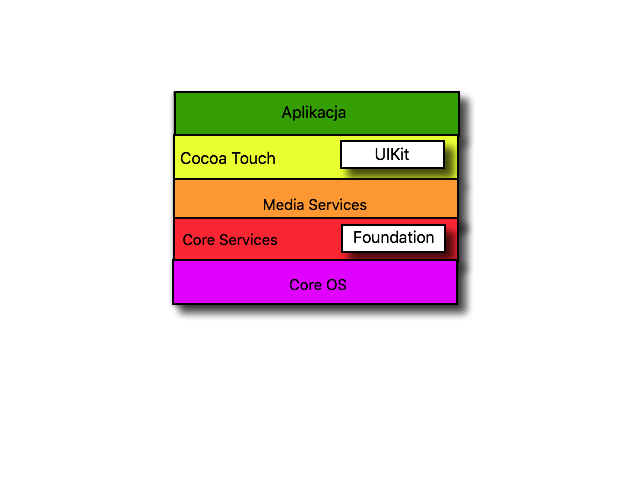
\includegraphics[scale=.5]{image/ArchitekturaiOS.jpg}
\caption{Architektura systemu iOS}
\label{fig:Architektura iOS}
\end{figure}
Architektura systemu \textit{iOS}  widoczna na rysunku \ref{fig:Architektura iOS} wywodzi się z \textit{Mac OS X}  oraz na przenośnym interfejsie systemu operacyjnego \textit{UNIX}. Stworzony jest na bazie czterech warstw abstrakcji: \textit{Core OS}, \textit{Core Services}, \textit{Media Services}, \textit{Cocoa Touch}.

\textit{Core OS} jest jądrem systemu operacyjnego, czyli bazowa warstwa systemu obsługująca bezpośrednio sprzęt. Odpowiedzialna jest między innymi za przetwarzanie obrazów, Bluetooth, dźwięk, DNS (ang. Domain Name System ), prywatne lub publiczne klucze, system obsługujący wątki, zarządzanie pamięcią.

\textit{Core Services} -- podstawowe usługi systemowe, które są podzielone na rożne biblioteki napisane w języku C i \textit{Objective-C}. Najważniejszymi bibliotekami przekazanymi w \textit{Core Services} są:
\begin{itemize}
\item \textbf{Foundation Framework} -- Podstawowa biblioteka stosowana w \textit{Objective-C} zawierająca zestawy klas przyśpieszające prace z językiem. Klasy tej biblioteki zaczynają się od liter \textit{NS} co jest skrótem od nazwy systemu \textit{NextStep}.
\item \textbf{Core Foundation Framework} -- biblioteka oparta na języku programowania C i pozwala na pracę z typami danych, kolekcjami oraz obsługę tekstowego typu znaków.
\item \textbf{Core Data Framework} -- biblioteka, która pozwala na zarządzanie modelem przechowywania danych. Zapewnia ogólne i automatyczne rozwiązanie typowych zadań związanych cyklem życia obiektów, zarządzanie wykresem obiektów, zapewnia sprawdzanie czy dane mają poprawne typy, sprawdza spójność między relacjami.
\item \textbf{Core Location Framework} -- rejestruje informacje o położeniu przy pomocy GPS czy sieci WiFi.
\end{itemize} 
\textit{Media Services} jest warstwą odpowiedzialną za renderowania grafiki, tekstu czy obsługę dźwięku. Do najważniejszych bibliotek tej warstwy można zaliczyć \textit{Core Audio}, \textit{Core Animation}, \textit{Core Text} oraz wydajnym środowiskiem pozwalającym renderowanie grafiki 2D \textit{Core Image}.

Główną biblioteką warstwy \textit{Cocoa Touch} jest \textit{UIKit}, czyli framework napisany w języku \textit{Objective-C} dostarczający różne funkcjonalności potrzebne do stworzenia interfejsu użytkownika dla aplikacji \textit{iOS}. Zawiera także zestaw instrukcji przydatnych w tworzeniu wielowątkowych aplikacji, obsługi dotyku, notyfikacji, czy dostęp do danych urządzenia.

\subsection{Możliwości developerskie w iOS}
W chwili pisania tej pracy najnowszym system operacyjnym jest \textit{iOS 9}, czyli dziewiąty z kolei większe uaktualnienie mobilnego systemu operacyjnego na urządzenia firmy \textit{Apple}. Został zaprezentowany pierwszy raz na konferencji \textit{Apple Worldwide Developers Conference} 8 czerwca  2015 roku, zaś dostępny na urządzeniach od 16 września tego samego roku. W porównaniu ze swoim poprzednikiem \textit{iOS 8} skoncentrowany był bardziej na optymalizacji działania urządzenia takiego jak wydłużenie pracy baterii aniżeli dodanie nowych funkcjonalności do systemu. 

Wraz z nowym system \textit{iPad} zyskał możliwość obsługiwania dwóch aplikacji jednocześnie. Funkcja \textit{Slide Over} pozwala użytkownikowi wybrać inna aplikacje od tej, którą w danej chwili używa oraz szybką interakcję z nią. Zaś \textit{Split View} daję możliwość uruchomienia dwóch aplikacji jednocześnie obok siebie na urządzeniu \textit{iPad Air 2}. Funkcja \textit{Picture in Pricture} pozwala użytkownikowi wyświetlanie okienka z treścią wideo podczas wykonywania innych czynności na urządzeniu. Choć to użytkownik decyduje kiedy chce korzystać z dwóch aplikacji w tym samym czasie, deweloper nie ma kontroli kiedy to następuję, musi on jednak pamiętać o dwóch rzeczach przy tworzeniu aplikacji by zapewnić użytkownikowi jak najlepsze doświadczenie z wielozadaniowością. Pierwszą jest by aplikacja zarządzała w efektywny sposób zasobami pamięci urządzenia kiedy dzieli system z drugą aplikacją. Gdy występuję ostrzeżenie o braku pamięci system prewencyjnie zabija aplikacje, która zużywa najwięcej pamięci. Drugą sprawą jest zaadoptowanie odpowiednich wielkości dla interfejsu by wszystko wyglądało poprawnie gdy użytkownik zdecyduje współdzielić ekran z inną aplikacją.  

\textit{3D Touch} daję użytkownikom dodatkową interakcje z urządzeniem poprzez siłę nacisku dotyku. Na urządzeniach obsługujących tę funkcjonalność możemy wybrać odpowiednie zadania aplikacji takie jak podgląd elementu, otworzenie w innym oddzielnym widoku,  poprzez naciśnięcie ikonki programu w głównym ekranie telefonu. Do obsługi tej funkcjonalności dostarczone zostały \textit{API} takie jak:
\begin{itemize}
\item \textbf{UIApplicationShortcut} -- pozwala na dodanie skrótu aplikacji na ekran główny telefonu wraz dodatkowymi funkcjonalnościami.
\item \textbf{UIKit peek and pop} -- to \textit{API} pozwalające w łatwy sposób uzyskać dostęp do dodatkowych treści w obrębie aplikacji.
\item \textbf{WebView peek and pop} -- umożliwia pogląd strony \textit{HTML} poprzez link prowadzący do tej strony.
\item \textbf{UITouch} -- dla określonej siły nacisku można przypisać rożne interakcje z użytkownikiem.
\end{itemize}
Obojętnie które z tych nowych funkcjonalności użyjemy, developer piszący aplikacje  musi sprawdzić czy urządzenie jest kompatybilne z funkcją \textit{3D Touch},na ten moment jedynie modele 6s i 6s Plus obsługują ten dodatek.

\textit{App Thining} jest nowym rozwiązaniem firmy \textit{Apple} by użytkownicy ściągali tylko takie komponenty aplikacji potrzebne do jej uruchomienia jakie odpowiadają konkretnemu typowi urządzenia. Np. urządzenia typu IPhone (4s, 5, 5s, 6) ściągać będą tylko grafiki odpowiadające temu typowi zamiast pobierać dodatkowe elementy potrzebne dla urządzeń typu \textit{HD} np. IPad, co skutkować będzie mniejszymi aplikacjami, szybszym ściąganiem i zadowolonymi użytkownikami. Wraz z środowiskiem Xcode 7 mamy możliwość przesłania aplikacji do \textit{iTunes} w pośrednim stanie zwanym Bitcode. W stanie takim kiedy użytkownik będzie chciał pobrać aplikacje, App Store automatycznie stworzy optymalną wersje tej aplikacji(jeśli potrzebna wersje 64--bitową) do pasującego urządzenia\footnote{\url{https://developer.apple.com/library/ios/releasenotes/General/WhatsNewIniOS/Articles/iOS9.html} czas dostępu:  2016-04-21}. 


\section{Środowisko programistyczne Xcode}
\textit{Xcode} jest zintegrowanym środowiskiem programistycznym (ang. \textit{Integrated Development Environment}, IDE), inaczej zestawem narzędzi developerskich potrzebnych do stworzenia aplikacji (w szczególności edytor tekstu, kompilator, narzędzie do debugowania, emulator urządzeń iOS), łączy wszystko w jeden pakiet oprogramowania zamiast kilka odrębnym narzędzi połączonych ze sobą skryptem. \textit{Xcode} jest też oficjalnym IDE \textit{Apple'a} do programowania aplikacji na Mac oraz iOS. Pierwotnie znany był jako \textit{Project Builder} w czasach kiedy jeszcze firma Apple istniała pod nazwą \textit{NeXT}, wraz z systemem operacyjnym Mac OS X 10.3 zmieniono nazwę na \textit{Xcode}. Zapewnia wsparcie dla języków programowania takich jak C, C++, Objective-C, Objective-C++, Java, AppleScript, Python, Ruby, Rez oraz Swift, dopuszcza także kompilację w modelach programowania \textit{Cocoa}, \textit{Carbon} i Java.
\begin{figure}[!th]
\centering
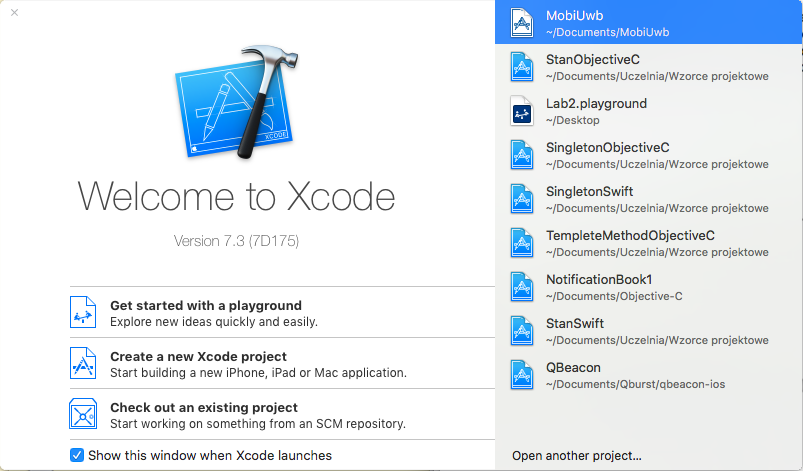
\includegraphics[scale=.5]{image/XcodeOknoPowitalne.png}
\caption{Okno powitalne przy uruchomieniu Xcode}
\label{fig:XcodeOknoPowitalne}
\end{figure}

Okno widoczne na rysunku \ref{fig:XcodeOknoPowitalne} jest pierwszym oknem pojawiającym się przy każdym uruchomieniu  \textit{Xcode} przy użyciu ikony programu. Po prawej stronie okna wyszczególniona została lista ostatnio utworzonych projektów oraz ich ścieżkę dostępu. Po lewej stronie oprócz nazwy programu wraz z jego wersją dostępne są trzy opcje. Pierwszą z nich jest rozpoczęcie pracy z plikiem typy \textit{playground}, jest to funkcja pozwalająca w szybki i łatwy sposób przetestować kod bez konieczności tworzenia projektu oraz poświęcaniu uwagi kompilacji. Drugą opcją jest utworzenie nowego projektu \textit{Xcode} na urządzeniu typu iPhone, iPad czy Mac. Trzecią opcją jest rozpoczęcie pracy nad istniejącym projekcie poprzez skopiowanie go z repozytorium po uprzednim podaniu wymagających danych typu login, hasło czy link do repozytorium.

\begin{figure}[!th]
\centering
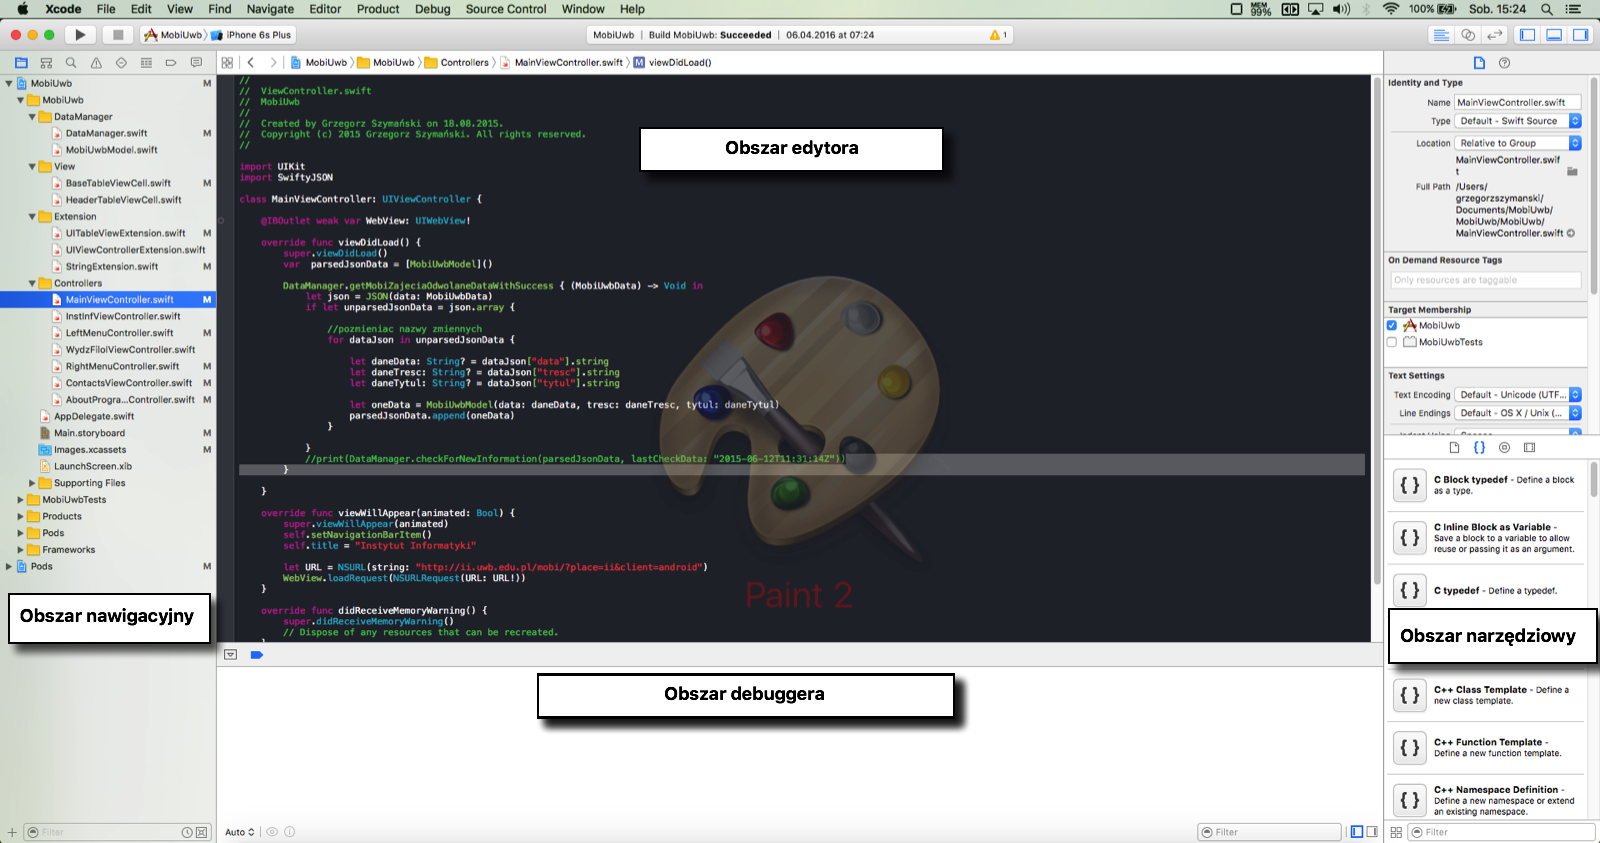
\includegraphics[scale=.3]{image/XcodeOknoProgramu.png}
\caption{Okno programu Xcode po uruchomieniu projektu}
\label{fig:XcodeOknoProgramu}
\end{figure}

Rysunek \ref{fig:XcodeOknoProgramu} przedstawia cztery obszary umożliwiające sprawną pracę nad tworzonym projektem. Obszar nawigacyjny daje dostęp do plików, klas, testów czy diagnostyki. Pasek nawigacyjny widoczny na rysunku \ref{fig:XcodeNavigationBar} umożliwia nam:
\begin{itemize}
\item \textbf{Projekt navigator} -- dodaje, usuwa, grupuje i zarządza plikami projektu. Pozwala na zaznaczeniu interesującego nas pliku i wyświetlenie w obszarze edytora. 
\item \textbf{Symbol navigator} -- wyświetla wszystkie klasy projektu jako listę lub hierarchie.
\item \textbf{Find navigator} -- pozwala na wyszukanie ciągu znaków w projekcie. 
\item \textbf{Issue navigator} -- pokazuje diagnostykę, ostrzeżenia, błędy, które pojawiają się po zbudowaniu projektu.
\item \textbf{Test navigator} -- tworzy, zarządza i uruchamia test aplikacji.
\item \textbf{Debug navigator} -- daje możliwość obsługiwania podstawowych narzędzi do debugowania.
\item \textbf{Breakpoint navigator} -- wyświetla wszystkie ustawione punkty przerwania oraz wbudowane opcje np. wyłapujące wszystkie wyjątki.
\item \textbf{Report navigator} -- umożliwia przeglądanie logów tworzonych podczas działania programu jak również uruchamiania aplikacji.
\end{itemize}
\begin{figure}[!th]
\centering
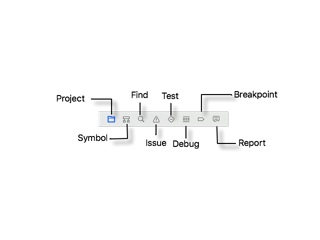
\includegraphics[scale=.7]{image/XcodeNavigationBar.png}
\caption{Pasek nawigacyjny}
\label{fig:XcodeNavigationBar}
\end{figure}

Zawsze widocznym obszarem okna \textit{Xcode} jest edytor kodu przyśpieszający prace poprzez udostępnienie wielu funkcjonalnych możliwości, takich jak rozpoznanie i wyróżnienie składni, generowanie wcięć, sugerowanie i autouzupełnianie kodu. Umieszczony w prawym górnych rogu przycisk uruchamiający \textit{Assistant Editor} dzieli edytor na dwie części, które pozwalają otworzyć dwa oddzielne dokumenty jednocześnie. Na przykład gdy edytujemy plik \emph{MojaKlasa.m} w nadrzędnym edytorze, \textit{Assistant Editor} automatycznie otworzy plik związany z naszą klasa \emph{MojaKlasa.h}.

Obszar narzędziowy możemy podzielić na dwa odrębne panele. Pierwszy z nich umiejscowiony na górze nazywa się panelem Inspektora i zawiera informację takie jak ścieżka dostępu do pliku, kodowanie tekstu czy danych o systemie kontroli wersji. Panel dolny nazywany panelem Bibliotek dzieli się na cztery elementy zawierające wszystkie pliki multimedialne użyte w projekcie, funkcje i kontrolki biblioteki \textit{Cocoa Touch}, gotowe schematy klas, widoków i kontrolerów oraz zakładkę \textit{Code Snippets} z kawałkami kodów, który można użyć wielokrotnie.

Ostatnim z obszarów z których zbudowane jest okno programu \textit{Xcode} jest obszar debuggera. Kontroluje on wykonanie naszego kodu, wyświetla utworzone zmienne czy wyjściowe parametry w konsoli. Składa się z trzech głównych komponentów:
\begin{itemize}
\item \textbf{Pasek debuggera} -- kontroluje wykonywanie się aplikacji i zapewnia nawigację po kodzie źródłowym. 
\item \textbf{Sektor widoku zmiennych} -- wyświetla informacje na temat elementów zaznaczonych na pasku debuggera.
\item \textbf{Sektor konsoli} -- zawiera interaktywny terminal.
\end{itemize}

\begin{figure}[!th]
\centering
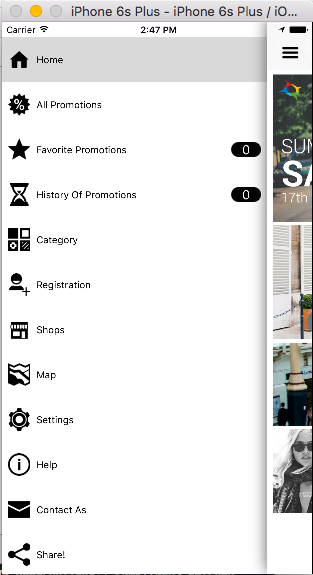
\includegraphics[scale=.7]{image/XcodeSymulator.png}
\caption{Symulator urządzenia programu Xcode}
\label{fig:XcodeSymulator}
\end{figure}
Widoczny na rysunku \ref{fig:XcodeSymulator} zrzut ekranu przedstawia symulator urządzeń programu \textit{Xcode}. Pozwala on w szybki sposób zbudować i przetestować aplikacje w trakcie jej pisania. Zainstalowany jest jako narzędzie \textit{Xcode}, uruchamia się na naszym komputerze jako aplikacja ale działa jak standardowe urządzenie mobilne typu iPhone, iPad, Apple Watch\footnote{iPhone -- telefon firmy Apple, iPad -- tablet firmy Apple oraz Apple Watch -- zegarek}. Umożliwia symulowanie iOS, watchOS czy tvOS w wybranej przez wersji systemów. Każda wersja i rodzaj urządzenia na którym symulujemy aplikacje traktowane jest jak oddzielne środowisko z niezależnymi ustawieniami i plikami systemowymi. Dzięki symulacji poprzez te narzędzie jesteśmy w stanie znaleźć błędy w aplikacji jeszcze na etapie konstruowania i wczesnych testów.

Przy tworzeniu aplikacji może pojawić się problem z widokiem czy ustawieniami \textit{auto layout constraints}, który trudno znaleźć poprzez przeglądanie kodu. Zamiast próbować wizualizować sobie układ obiektów \textit{Xcode} dostarcza nam narzędzie pokazujące całą hierarchie widoku widoczną na rysunku \ref{fig:XcodeViewHierarchy}. \textit{Xcode} robi zrzut ekranu i prezentuje w trójwymiarze interfejs użytkownika czyli pozycje,kolejność i wielkość każdego z elementów widoku oraz jak na siebie wzajemnie oddziałują.

 \begin{figure}[!th]
\centering
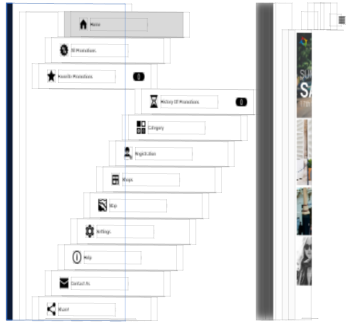
\includegraphics[scale=.5]{image/XcodeViewHierarchy.png}
\caption{Hierarchia widoku aplikacji}
\label{fig:XcodeViewHierarchy}
\end{figure}
\section{Języki programowania}
Język programowania, informatyczne narzędzie do formułowania programów dla komputerów; jest językiem formalnym, którego składnia określa zasady zapisu programów (w sposób jednoznaczny i łatwy do analizy), a semantyka przypisuje programom ich interpretację (określa efekty działania programu zapisanego w języku programowania).

Składnia języka programowania jest najczęściej definiowana za pomocą gramatyki bezkontekstowej (gramatyka formalna), w której można wygodnie opisać zagnieżdżone struktury (np. instrukcje złożone, wyrażenia arytmetyczne z nawiasami); dodatkowe warunki składniowe, których nie można zdefiniować w ten sposób (np. wymaganie, aby funkcje użyte w programie były w nim zdefiniowane), są najczęściej zapisywane w języku naturalnym. Semantyka jest zwykle opisywana tekstem w języku naturalnym, choć można ją określić w sposób w pełni precyzyjny i formalny, np. podając reguły tłumaczenia konstrukcji języka programowania na ciąg operacji pewnego hipotetycznego komputera (semantyka operacyjna) albo określając sposób konstruowania funkcji przekształcającej dane wejściowe programu w jego wyniki (semantyka denotacyjna)\footnote{\url{http://encyklopedia.pwn.pl/haslo/jezyk-programowania;3917948.html} czas dostępu:2016-04-21}. 
\subsection{Objective-C}
\textit{Objective-C} jest jednym z dwóch języków programowania używanym do tworzenia oprogramowania na platformy OS X, iOS czy watchOS. Pochodzi on od języka C i dziedziczy takie elementy jak np. składania, typy prymitywne oraz instrukcje sterujące, co więcej kod poprawnie napisany języku C jest kompatybilny i zgodny z językiem \textit{Objective-C}, choć rozszerzony jest o możliwości programowania obiektowego pochodzące od \textit{Smaltalka}.
W 1988 firma \textit{NeXT Software} wykupiła licencje do tego języka i wypuściła bibliotekę opartą o język \textit{Objective-C} pod nazwą \textit{NeXTSTEP}. Kiedy firma \textit{Apple} została właścicielem \textit{NeXT}, bibliotekę wbudowano w jądro systemów operacyjnych \textit{Mac OS X}, zapewniając tym sposobem nowoczesny fundament OS, którego \textit{Apple} nie było w stanie zapewnić we własnym zakresie.

W \textit{Objective-C} wymaga się by deklaracja i definicja klasy odbywała się w dwóch odrębnych plikach. Przyjęło się by deklarację umieszczać w pliku nagłówkowym z rozszerzeniem .h i między słowem kluczowym \textit{@interface} oraz zamykającym \textit{@end} widoczne na listingu \ref{Deklaracja klasy w Objective-C}. Zadeklarowana klasa posiada dwa parametry typu NSObject(klasy bazowej większości klas języka \textit{Objective-C}), przedrostek NS wymienionych typów parametrów pochodzi od biblioteki \textit{NeXTSTEP}, która została wspomniana wcześniej. Od wiersza 6 do 12 widoczne są metody klasy oraz metody instancji, \textit{"+"} oznacza metodę klasy, dzięki niej nie potrzebujemy tworzyć instancji klasy by wywołać tą metodę. Drugi rodzaj metody operuje na stworzonym obiekcie danej klasy.
\begin{lstlisting}[label=Deklaracja klasy w Objective-C, caption=Deklaracje klasy w umieszczamy w pliku z rozszerzeniem \textit{.h}]
@interface NazwaKLasy: klasaNadrzedna {
	NSObject *parametr1Klasy
	NSObject *parametr2Klasy
}

+ (void)metoda1Klasy;
+ (typParametruWyjsciowego) metoda2Klasy;
+ (typParamteruWyjsciowego) metoda3Klasy:(typParametruWejsciowego) nazwaParametruWejsciowego;

- (void)metoda1Instancji;
- (typParametruWyjsciowego) metoda2Instancji;
- (typParamteruWyjsciowego) metoda3Instancji:(typParametruWejsciowego) nazwaParametruWejsciowego;

@end
\end{lstlisting}

W sekcji drugiej nazywanej definicją klasy, kod umieszczony w pliku z rozszerzeniem \textit{.m} odpowiedzialny jest za rzeczywiste działanie klasy. Definicje metod umieszczamy między słowem kluczowym \textit{@implementaion} a zamykającym \textit{@end}. W przypadku metody widocznej na listingu\ref{Definicja klasy w Objective-C} by nie wyskoczył błąd przy kompilacji typ parametru wyjściowego musi być taki sam jak w przypadku parametru wejściowego.
\begin{lstlisting}[label=Definicja klasy w Objective-C, caption=Definicje klasy w Objective-C umieszczamy w pliku z rozszerzeniem .m]
@implementation
-(typParametruWyjsciowego) metoda2instancji:(typParamteruWejsciowego) nazwaParametruWejsciowego {
	return ParamertWejsciowy
}
@end
\end{lstlisting}

Zazwyczaj do stworzenie obiektu danej klasy potrzebujemy dwóch metod. Pierwsza z nich widoczna w listingu \ref{StworzenieObiektu} nazywa się \textit{allloc} i odpowiada za przydzielenie odpowiedniej wielkości na obiekt w pamięci naszego komputera, zaś druga \textit{init} jest domyślnym konstruktorem gdy nie nadpiszemy go sami dziedziczony jest z klasy nadrzędnej \textit{NSObject}.
\begin{lstlisting}[label=StworzenieObiektu, caption=Instrukcja stworzenia obiektu.]
NaszaKlasa * nazwaKlasy = [[NaszaKlasa alloc] init];
\end{lstlisting}

Obiekty klas powinny mieć wyraźnie zdefiniowane zadania, pozwalające na  wykonywanie określonych czynności takich jak modelowanie konkretnej informacji, wyświetlenia treści, kontrole przepływu informacji. Interfejs klasy definiuje sposoby dzięki którym poprzez spodziewaną interakcje na obiekcie jesteśmy w stanie osiągnąć te czynności. Niekiedy jednak potrzebujemy rozszerzyć funkcjonalność klasy poprzez dodanie nowej metody czy parametru by bardziej odpowiadała naszym potrzebom. Dla przykładu, możemy potrzebować by nasza aplikacja wyświetlała konkretny ciąg znaków kilkanaście razy w różnych miejscach, zamiast tworzyć obiekty za każdym razem gdy będziemy potrzebować tej funkcjonalności możemy wziąć pod uwagę czy nie dodać jej do klasy \textit{NSString} by to ona mogła to wyświetlić ten napis. Stworzenie podklasy dziedziczącej z \textit{NSString} ogranicza tą funkcjonalność i użycie jej type \textit{NSMutableString} będzie już niemożliwe. Zamiast tego \textit{Objective-C} daje nam możliwość dodanie własnych metod do istniejących klas poprzez kategorie i rozszerzenia klas. 

Jeśli potrzebujemy dodać metody do już istniejącej klasy najprostszym sposobem jest dodanie kategorii. Zaczynamy od deklaracji nagłówka wraz z zainicjowaniem metody widocznej w wierszu 5,oraz nazwy kategorii wyszczególnionej w nawiasach obok nazwy klasy widocznej w wierszu 3 listingu \ref{KategoriaNaglowek}.
\begin{lstlisting}[label=KategoriaNaglowek, caption=Deklaracja nowej metody poprzez kategorie]
#import "Osoba.h"

@interface Osoba (OsobaWypiszDaneOsobowe)

-(NSString *) wypiszNazwiskoImie;
}

@end
\end{lstlisting}
Następnym krokiem jest zaimplementowanie funkcjonalności naszej metodzie. Przyjęło się by plik kategorii nazywać poprzez połączenie przez ""+"" nazwę klasy do której dodajemy kategorie oraz nazwę opisującą kategorie widoczną na listingu \ref{KategorieImplementacja} w wierszu 1. Teraz wystarczy tylko zaimportować tę klasę gdy będziemy potrzebowali skorzystać z nowej funkcjonalności.
\begin{lstlisting}[label=KategorieImplementacja, caption=Definicja metody kategorii]
#import "Osoba+OsobaWypiszDaneOsobowe.h"

@interface Osoba (OsobaWypiszDaneOsobowe)

-(NSString *) wypiszNazwiskoImie {
	return [NSString stringWithFormat:@"%@, %@", self.nazwisko, self.imie];
}

@end
\end{lstlisting}
Rozszerzenia klasy działają podobnie jak kategorie, z tą różnicą że dodać je możemy tylko do klas których posiadamy kod źródłowy (kompilacja klasy odbywa się w tym samym czasie co rozszerzenie tej klasy). Składania pozwalająca na deklaracje rozszerzenia klasy widoczna na listingu \ref{RozszerzeniaKlasy} jest bardzo podobno do składni kategorii. Ponieważ nie podana jest żadna nazwa w nawiasach w wierszu 1 rozszerzenia nawiązują to kategorii anonimowej. W przeciwieństwie do zwykłych kategorii, rozszerzenie daje nam możliwość dodania \textit{@property} czy zmiennych instancji widocznej w wierszu 3. Kompilator automatycznie syntetyzuje zmienną instancji do implementacji klasy podstawowej.

\begin{lstlisting}[label=RozszerzeniaKlasy, caption=Deklaracja nowego parametru poprzez rozszerzenie klasy bazowej]
@interface Osoba ()

@property NSString  *adres; 

@end
\end{lstlisting}

Protokoły \cite{Kohan:2012:Obj} to lista metod wspólnie użytkowane przez klasy. Metody znajdujące się na takiej liście nie mają implementacji, ponieważ są przeznaczone do zaimplementowania przez innych programistów. Określany jest jako sposób definicji zestawu metod, które mają jakiś związek z określoną nazwą. Metody te zazwyczaj są dobrze udokumentowane, dzięki czemu wiadomo, jak mają działać i można je w razie potrzeby zaimplementować w swojej klasie. Może zawierać listę metod, których implementacja jest opcjonalna, oraz zestaw takich, które trzeba zaimplementować obowiązkowo. Jeśli zaimplementuje się wszystkie wymagane metody, mówi się, że klasa jest zgodna z danym protokołem lub go adaptuje. Można zdefiniować zarówno protokół zawierający same wymagane, jak i same opcjonalne metody. Składnia definicji protokołu widoczna na listingu \ref{Protokol} jest dosyć prosta, należy użyć dyrektywy \textit{@protocol}, po której wpisuje się dowolną nazwę definiowanego protokołu. Następnie deklaruje się metody w taki sam sposób jak w sekcji interfejsu. W skład protokołu wchodzą wszystkie metody zadeklarowane między słowami \textit{@protocol} i \textit{@end}.

\begin{lstlisting}[label=Protokol, caption=Protokół \textit{NSCopying} zdefiniowany w pliku nagłówkowym \textit{NSObject.h}]
@protocol NSCopying

- (id)copyWithZone: (NSZone *)zone;

@end
\end{lstlisting}

Czasami zachodzi potrzeba by parametr naszej klasy raz zainicjowany zachował swoją wartość pomimo iż został wywoływany kilkakrotnie lub ograniczyć widoczność funkcji tylko do pliku gdzie została zdefiniowana. W obu przypadkach słowem kluczowym odpowiedzialnym za te funkcjonalności jest komenda \textit{static}.
\begin{lstlisting}
int liczCoTrzy() {
	static int licznik = 0;
	licznik += 3;
	return licznik
}

int main() {
	liczCoTrzy(); // 3
	liczCoTrzy(); // 6
	liczCoTrzy(); // 9
	return 0;
}
\end{lstlisting}
Zmienna statyczna \textit{licznik}, która została trzy razy zainicjowana zachowała swoją wartość z poprzednich wywołań co pozwoliło osiągnąć upragniony efekt.
Domyślnie wszystkie funkcje widoczność globalną, co oznacza że raz zdefiniowana funkcja w jednym pliku jest od razu widoczna we wszystkich innych. Słowo kluczowe \textit{static} pozwala ograniczyć widoczność funkcji do konkretnego pliku, dzięki temu możemy stworzyć funkcje prywatną i uniknąć konfliktów w nazwach.
\begin{lstlisting}
//deklaracja funkcji statycznej
static int dodajLiczby(int, int);

//Implemetacja funkcji statycznej
static int dodajLiczby(int pierwsza, int druga) {
	return pierwsza + druga;
}
\end{lstlisting}
Trzeba pamiętać by słowo kluczowe \textit{static} było użyte przy deklaracji i implementacji.
\subsection{Swift}
Swift \cite{Lassoff:2014:Swift} to opracowany przez \textit{Apple'a} nowy język programowania, który ma być przyjazny i łatwy w użyciu. Został zaprojektowany z uwzględnieniem filozofii łatwości użycia i szybkości działania języków skryptowych, a jednocześnie oferuje potężne możliwości charakterystyczne dla języków kompilowanych.	 Opracowany przez \textit{Apple'a} język \textit{Swift} został zaprezentowany w roku 2014, od tamtej chwili jest zintegrowany z \textit{Xcode} i pozwala na tworzenie aplikacji na platformy OS X, iOS oraz watchOS. 

W chwili pisania tej pracy \textit{Swift} dostępny jest w wersji 2.2 i wraz z nowym wydaniem wprowadzono kilka istotnych zmian poprawiających prace. Zdecydowano się na nowy model obsługi błędów widoczny na listingu \ref{ObslugaBledow}, który ma dostarczyć jasną i przejrzystą składnie obsługującą błędy. Nowy model błędów, który pozwala na stworzenie własnych typów błędu, został zaprojektowany do płynnej współpracy z \textit{NSError} i biblioteką \textit{Cocoa}.
\begin{lstlisting}[label=ObslugaBledow, caption=Nowy model obsługi błedów w Swift]
func wczytajDane() throws {}

func test() {
	do {
		try wczytajDane()
		} catch {
			print(error)
		}
}
\end{lstlisting}
Dodano nowe funkcje składniowe, które pomagają pisać bardziej przejrzysty kod, poprawiając jednocześnie jego spójność. Zastosowano w \textit{SDK} nowe funkcjonalności z \textit{Objective-C} takie jak typy generyczne czy wartości \textit{null} adnotacji poprawiające bezpieczeństwo kodu. Niektóre z pozostałych ulepszeń to:
\begin{itemize}
\item lepsza kontrola przepływu działania przy pomocy \textit{do}, \textit{guard}, \textit{defer} i \textit{repeat}.    
\item rozszerzenia protokołów i domyślna implementacja.
\item rozszerzone dopasowanie do wzorca do pracy klauzulą if i pętlą for.
\end{itemize}
Wraz z nową wersją pojawiła się informacja, że \textit{Swift} stał się oprogramowaniem \textit{open source}. W tym samym czasie otwarta została strona\footnote{\url{https://swift.org} czas dostępu: 2016-06-01} z dostępnym kodem, rejestratorem błędów i systematycznymi wersjami developerskimi dla każdego. Na razie \textit{Swift} obsługuje platformy \textit{Apple} oraz \textit{Linux} ale pracują na resztą platform.

Częścią wspólną dla zmiennych i stałych jest nazwa oraz wartość przechowywane określonego typu. Wartość stałej raz zainicjowanej nie może zostać zmieniona, w przeciwieństwie do zmiennych gdzie wartość może zostać zmieniona wielokrotnie. Podstawową zasadą jest by zadeklarować zmienne lub stałe przed próbą ich użycia. Słowem kluczowym za zadeklarowania stałej w języku \textit{Swift} odpowiada \textit{let}, zaś zmiennej \textit{var} widoczne na listingu \ref{StaleIZmienne}. Dobrym zwyczajem jest by właściwie deklarować stałe i zmienne, co nie tylko sprawia, że nasz kod jest bezpieczniejszy ale świadczy o znajomości pisanego przez nas kodu.
\begin{lstlisting}[label=StaleIZmienne, caption=Deklaracja stałych i zmiennych w Swift]
let stalaLiczbaPi = 3.14159

var zmiennaX = 10
\end{lstlisting}
W języku \textit{Swift} bardzo rzadko jesteśmy zmuszeni to definiowania typu po zainicjowaniu wartości dla zmiennej lub stałej. Prawie zawsze \textit{Swift} jest w stanie sam wywnioskować typ po wartości.

Funkcje są samodzielnymi kawałkami, które odpowiadają za wykonanie konkretnego zadania. Nazywamy funkcje zgodnie z jej wykonywanym zadaniem i wywołujemy tą nazwę w miejscu gdzie te konkretne zadanie ma być wykonane. Składnia funkcji w \textit{Swift} jest na tyle elastyczna, aby wyrazić wszystko, od prostych funkcji w stylu języka \textit{C} bez nazw parametrów wejściowych do kompleksowych metod \textit{Objective-C} z lokalnymi i zewnętrznymi nazwami dla każdego parametru. Możemy podać dla parametrów wejściowych wartości domyślne w celu uproszczenia wywołań funkcji lub użyć parametrów \textit{in-out}, które mogą być przekazane poza funkcje ze zmodyfikowanymi wartościami.
\begin{lstlisting}[label=Funkcje, caption=Definicja funkcji w języku Swift]
func przywitajSieZ(imieOsoby: String) -> String {
	
	let powitanie = "Witaj, " + imieOsoby + "!"
	
	return powitanie 
	
}

\end{lstlisting}
Funkcja widoczna na listingu \ref{Funkcje} nosi nazwę \textit{przywitajSieZ(\_:)}, ponieważ za to właśnie odpowiada -- bierze imię osoby i zwraca powitanie z tą osobą. By to osiągnąć zdefiniowaliśmy jeden parametr wejściowy typu \textit{String} i zwrócimy typ \textit{String} zawierający powitanie wraz z imieniem. Rezultat widoczny jest poniżej.
\begin{center}
	print(przywitajSieZ("Kamil")) // "Witaj, Kamil!"
\end{center}

\textit{Swift} dostarcza trzy główne typy kolekcji, tablice, słownik oraz zbiór do przechowywania elementów. Tablice są uporządkowaną kolekcja danych, zbiór natomiast nieuporządkowana kolekcją unikatowych danych, zaś słownik nieuporządkowaną kolekcją typu klucz--wartość. W żadnej z tych kolekcji nie możemy wstawić wartości o różnych typach, daje nam to pewność, że wartość którą chcemy odzyskać z kolekcji jest określonego typu. 
W \textit{Objective-C} jeśli zależało nam na strukturze, która raz zainicjowana elementami nie zostanie zmieniona byliśmy zmuszeni do użycia kolekcji o innej nazwie i funkcjonalności od struktury, która pozwalała na taką zmianę. W języku \textit{Swift} słowami kluczowymi oznaczającymi czy kolekcje możemy modyfikować lub nie, odpowiadają tak jak w przypadku zmiennych i stałych, \textit{let} i \textit{var.}
Pełna nazwa typu tablicy w \textit{Swift} piszemy \textit{Array<Element>}, gdzie \textit{Element} oznacza typ wartości dozwolony do przechowania w tej tablicy. Możemy także skorzystać ze skróconej wersji pisząc tylko \textit{[Element]}. Obydwie formy działają identycznie, choć wersja skrócona jest preferowana. 
\begin{center}
	var tablicaIntow = [Int]()
\end{center}
Komenda widoczna powyżej odpowiedzialna jest za stworzenie pustej tablicy przechowującej wartości typu całkowitego. Jak już wcześniej wspomniałem \textit{Swift} jest w stanie wywnioskować samemu jakiego typu wartości będą przechowywane w tablicy, dlatego też inicjalizacja bez podania typu jest poprawna.
\begin{center}
	var tablicaStringow = ["kot","pies","kaczka","leniwiec"]
\end{center}
Przy korzystaniu z tablicy \textit{Swift} zapewnia kilkanaście przydatnych funkcji pozwalających na łatwą obsługę. Najczęściej używane funkcje to:
\begin{itemize}
\item \textbf{array.count()} -- zwraca liczbę elementów w tablicy w postaci liczby całkowitej.
\item \textbf{array.isEmpty()} -- sprawdza czy tablica jest pusta, jeśli tak zwraca wartość boolowską \textit{true} w przeciwnym przypadku \textit{false}.
\item \textbf{array.append(\_:)} -- dodaje element na koniec tablicy.
\item \textbf{array.insert(\_:atIndex:)} -- dodaje element pod wskazany przez nas index.
\item \textbf{array.removeAtIndex(\_:)} -- usuwa element ze wskazanego indexu.
\item \textbf{array.removeLast()} -- usuwa ostatni element z tablicy.
\end{itemize}

Zbiór (ang. \textit{Set}) przechowuje unikatowe wartości tego samego typu w kolekcji w niezdefiniowanej kolejności. Możemy użyć zbioru zamiast tablicy jeśli kolejność jest dla nas bez znaczenia lub gdy potrzebujemy mieć pewność, że element pojawi się tylko raz. Innym wymogiem używania tej struktury jest typ przechowywanych wartości a dokładniej musi posiadać funkcje haszującą, która zwraca wartość \textit{hash}. Wartość \textit{hash} jest liczbą całkowitą i jest jednakowa dla wszystkich elementów, które są sobie równe. Wszystkie podstawowe typy w \textit{Swift}(takie jak \textit{String},  \textit{Int},  \textit{Double} czy \textit{Bool}) posiadają taką funkcje domyślnie i mogą być przechowywane w \textit{Set}. Składnia wygląda podobnie jak w przypadku tablicy, \textit{Set<Element>} gdzie \textit{Element} odpowiada z przechowywany typ. Jednak w przeciwieństwie do tablicy nie posiada skróconej wersji. 
\begin{center}
	var litery = Set<Characters>()
\end{center}
Nawiasy bez argumentów oznaczają wywołanie konstruktora, który stworzy pusty \textit{Set} typu \textit{Character}. Większość funkcji dostępnych dla tablicy możemy użyć na \textit{Set}, jednak posiada on unikatowe warte uwagi funkcje:
\begin{itemize}
\item \textbf{set.intersect(\_:)} -- porównuje dwa zbiory i zwraca nowy zawierający elementy wspólne dla obu.
\item \textbf{set.exclusiveOr(\_:)} -- nowy zbiór bez elementów wspólnych.
\item \textbf{set.union(\_:)} -- połączenie dwóch zbiorów razem z elementami wspólnymi.
\item \textbf{set.substract(\_:)} -- pozostawia tylko te elementy, które nie pojawiły się w drugim zbiorze.
\end{itemize}

Ostatnią kolekcją dostępną w \textit{Swift} jest słownik przechowujący związki pomiędzy kluczami a wartościami tych samych typów kolekcji z niezdefiniowanym porządkiem. Każda wartość jest połączona unikatowym kluczem, który zachowuje się jak identyfikator dla wartości w słowniku. Powinniśmy wykorzystywać słownik kiedy potrzebujemy wyszukiwać wartość po identyfikatorze, podobnie jak w rzeczywistym słowniku wyszukujemy definicje określonego słowa. Pełna deklaracja typu dla słownika wygląda podobnie jak w pozostałych przypadkach lecz posiada dwa argumenty, \textit{Dictionary<Key, Value>} gdzie \textit{Key} odpowiada za identyfikator dla wartości. Jak w przypadku tablicy, słownik posiada skróconą wersje zapisu \textit{[Key: Value]}, i tak jak w przypadku tablicy skrócona wersja jest wersją preferowaną.
\begin{center}
	var kodyPocztoweMiejscowosci = [String: String]()
\end{center}
Definicja tworzy pusty słownik przechowujący jako klucz kod pocztowy dla miasta jako wartości. Przykładowe przypisane do istniejącego już słownika wyglądało by następująco:  
\begin{center}
	kodyPocztoweMiejscowosci = ["18-300": ""Zambrów"", "16-010": ""Nowodworce"", "12524": "Berlin", "20355": "Hamburg"]
\end{center}
Do iteracji po słowniku możemy wykorzystać strukturę zwaną \textit{tuple} oraz pętle for widoczną za listing \ref{IteracjaPoSlowniku}
\begin{lstlisting}[label=IteracjaPoSlowniku, caption=Iteracja po słowniku z wykorzystaniem \textit{tuple} i pętli for.]
for (kodPoczotwy, nazwaMiejscowosci) in kodyPocztoweMiejscowosci {
		print(kodPocztowy + " " +  nazwaMiejscowosci)
		
}
\end{lstlisting}
\cleardoublepage
\chapter{Implementacja aplikacji}
\label{cha:Implementacja aplikacji}
Oprogramowanie \textit{MobiUwB} stworzone na system operacyjny \textit{iOS} w wersji 9.1 lub wyższy ma na celu dostarczenie wygodnego dostępu do informacji dla studenta \textit{Uniwersytetu w Białymstoku} posiadającego urządzenie mobilne firmy \textit{Apple}. W funkcjonalny sposób dostarcza zawartość umieszczaną na oficjalnej stronie internetowej \textit{Uniwersytetu w Białymstoku} wprost do smartfonu lub tabletu użytkownika, bez konieczności korzystania z przeglądarki. 
\section{Opis aplikacji MobiUwB}
Oprogramowanie mobilne \textit{MobiUwB} jest tak zwaną aplikacją hybrydową z tego względu, że łączy w sobie dwa sposoby tworzenia aplikacji mobilnych. Z jednej strony główne informacje wyświetlane są za pomocą strony \textit{WWW} odpowiednio skonstruowanej by użytkownik miał wrażenie korzystania z aplikacji natywnej. Z drugiej strony korzysta z funkcji natywnych takich jak notyfikacje czy rożne sposoby kontaktu z sekretariatem uniwersytetu. Podejście takie pozwala na łatwiejszą implementacje aplikacji pod różne systemy operacyjne.
\subsection{Zastosowania}
Do głównych zastosowań aplikacji mobilnej \textit{MobiUwB} należą:
\begin{itemize}
\item \textbf{Dostarczanie informacji} -- Wszystkie ważne informacje dostępne są z poziomu jednego widoku, który dzięki podziałowi na różne kategorie takie jak aktualności czy zajęcia odwołane w przystępny sposób dostarczany jest dla użytkownika. Oprócz aktualizowanych komunikatów zawsze pod ręką znajduje się plan zajęć dla wszystkich studentów wybranych wydziałów.
\item \textbf{Konfigurowalne notyfikacje} -- Powiadomienia dzięki, którym bez ingerencji użytkownika dostarczane są informacje. Notyfikacje możemy włączyć lub wyłączyć całkowicie. Ustawić z jakich kategorii wiadomości nas interesują, do wyboru mamy: aktualności, zajęcia odwołane, sprawy ogólne, biuro karier oraz szkolenia i praktyki. Ostatnią opcją jest zmiana częstotliwości z jaką aplikacja ma sprawdzać czy nowa informacja pojawiła się w wybranym dziale.
\item \textbf{Łatwy kontakt z Uniwersytetem} -- Możliwość skontaktowania się z Uniwersytetem za pomocą jednego przycisku. Do wyboru mamy kontakt telefoniczny lub poprzez wysłania wiadomości e-mail. Dostępny jest także adres, który można wyświetlić w postaci lokalizacji \textit{GPS}.
\item \textbf{Grupowanie informacji} -- Informacje podzielone są na sześć grup: aktualności, zajęcia odwołane, sprawy ogólne, biuro karier, szkolenia i praktyki oraz plan zajęć. Od użytkownika zależy, z której grupy wiadomości go interesują wystarczy, że w głównym widoku aplikacji wybierze podział a strona odpowiednio wyświetli szukane informacje.
\end{itemize}

\subsection{Funkcje}
Jedną z najważniejszych klas odpowiedzialną za dostarczenie użytkownikowi notyfikacji o nowych informacjach w wybranych kategoriach jest \textit{AnnouncementManager}. Przy tworzeniu tej klasy wybrałem wzorzec projektowy \textit{singleton} (implementacja widoczna na listingu \ref{AnnouncementManager} w wierszu 3), który pozwala na stworzenie tylko jednej instancji tej klasy. Dzięki temu mamy pewność ze w całej aplikacji istnieje tylko jeden obiekt odpowiedzialny za sprawdzanie czy pojawiła się nowa wiadomość na serwerze oraz że obiekt nie zostanie zniszczony przy przechodzeniu do różnych widoków. Funkcja \textit{newAnnouncementsInCategory(\_:)} (wiersz 10-33) jako parametr wejściowy przyjmuje typ \textit{String} odpowiedzialny za wybraną przez użytkownika kategorie. Z tym parametrem wywoływana jest \textit{dateOfLastAnnouncementsOfCategory(\_:)}, która jest funkcją asynchroniczną odpowiadającą za połączenie z serwerem oraz zwrócenie daty ostatniego ogłoszenia. W dalszej części zwrócona oraz przekonwertowana data do odpowiedniego formatu porównywana jest z datą ostatniego sprawdzania. Data ta pobrana jest z \textit{userDefaults}, który jest słownikiem  przechowującym ustawienia oraz innych potrzebnych informacji o aplikacji. W przypadku gdy \textit{lastAnnouncementDate} jest nowsza od daty ostatniego sprawdzenia wywoływana jest funkcja \textit{sendNotificationForCategory(\_:)}, która wyświetla powiadomienie dla użytkownika odpowiednie dla wybranej kategorii. Końcową czynnością tej funkcji jest przypisanie do zmiennej \textit{lastCheck} timestampa\footnote{Timestamp -- jest sekwencją znaków przedstawiającą kiedy wybrane wydarzenie zaistniało.} oraz zapisanie wyniku do słownika \textit{userDefault} pod indeksem \textit{lastCheck}.
\newpage
\begin{lstlisting}[label=AnnouncementManager, caption=Klasa AnnouncementManager]
class AnnouncementManager {
    
    static let sharedInstance = AnnouncementManager()
    
    
   private init() {

    }
    
    func newAnnouncementsInCategory(category:String) {
        
        
        dateOfLastAnnouncementsOfCategory(category) { completion in
            if let lastAnnouncementDate = self.parseAnnouncementDate(completion) {
                var lastCheck:NSDate
                if let lastCheckedDate:NSDate = self.userDefaults.objectForKey("lastCheck") as? NSDate {
                    lastCheck = lastCheckedDate
                } else {
                    lastCheck = NSDate()
                }
                let compare = lastAnnouncementDate.compare(lastCheck)
                if compare == .OrderedDescending {
                    self.sendNotificationForCategory(category)
                }
                lastCheck = NSDate()
                self.userDefaults.setObject(lastCheck, forKey: "lastCheck")
            }
            
            
        }
        
    }
@end
\end{lstlisting}
\newpage
\begin{figure}
\centering
\begin{minipage}{.5\textwidth}
  \centering
  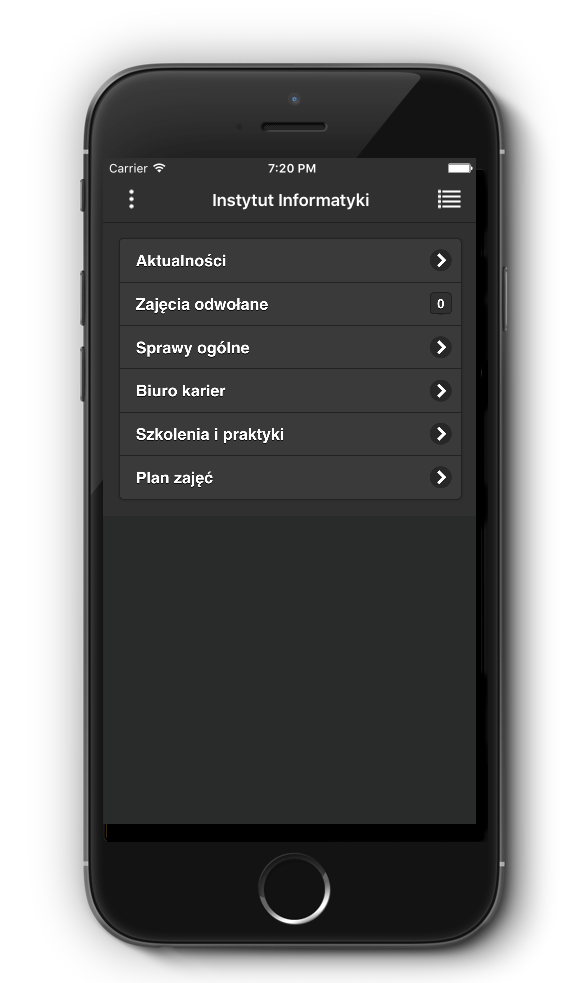
\includegraphics[width=.6\linewidth]{image/HomeIphone.png}
  \captionof{figure}{Ekran główny}
  \label{fig:Home}
\end{minipage}%
\begin{minipage}{.5\textwidth}
  \centering
  \includegraphics[width=.6\linewidth]{image/KontaktIphone.png}
  \captionof{figure}{Ekran kontaktu}
  \label{fig:Kontakt}
\end{minipage}
\end{figure}
\subsection{Elementy}
Aplikacja \textit{MobiUwB} na iOS składa się z wielu elementów, które w większości ukryte są dla użytkownika pod interfejsem graficznym ale połączeniu ze sobą komponują się w mobilną aplikacje. Interfejs ten składa się głownie z ekranów aplikacji, które można podzielić na :
\begin{itemize}
\item \textbf{Ekran główny} -- jest pierwszy interaktywny ekran jaki użytkownik widzi po włączeniu aplikacji. Składa się z dwóch elementów \textit{navigation bar} oraz \textit{web view}. Pierwszy z elementów zawiera dwa \textit{navigation items} na przeciwległych końcach belki odpowiedzialnych na wysuwane menu przedzielone tytułem zmieniającym się w zależności od ekranu. Całości dopełnia wyświetlana strona \textit{WWW} mieszcząca się w elemencie \textit{web view}.Ekran zaprezentowana jest na rysunku \ref{fig:Home}.
\item \textbf{Wysuwane menu} -- Rysunek \ref{fig:Menu} przedstawia lewe i prawe wysuwane menu dzięki, którym użytkownik może swobodnie nawigować po aplikacji. Prawe menu odpowiedzialne jest za przełączanie po wydziałach uniwersytetu zaś lewe menu zawiera listę ekranów dostępnych dla użytkownika.
\end{itemize}
\begin{figure}
\centering
\begin{subfigure}{.5\textwidth}
  \centering
  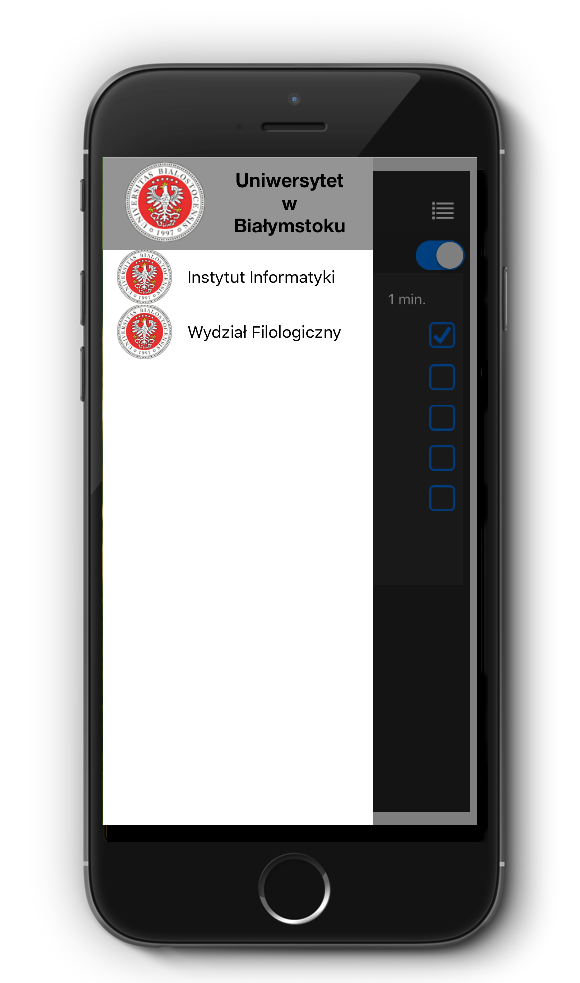
\includegraphics[width=.6\linewidth]{image/LeweIphone.png}
  \caption{Lewe menu}
  \label{fig:Lewe}
\end{subfigure}%
\begin{subfigure}{.5\textwidth}
  \centering
  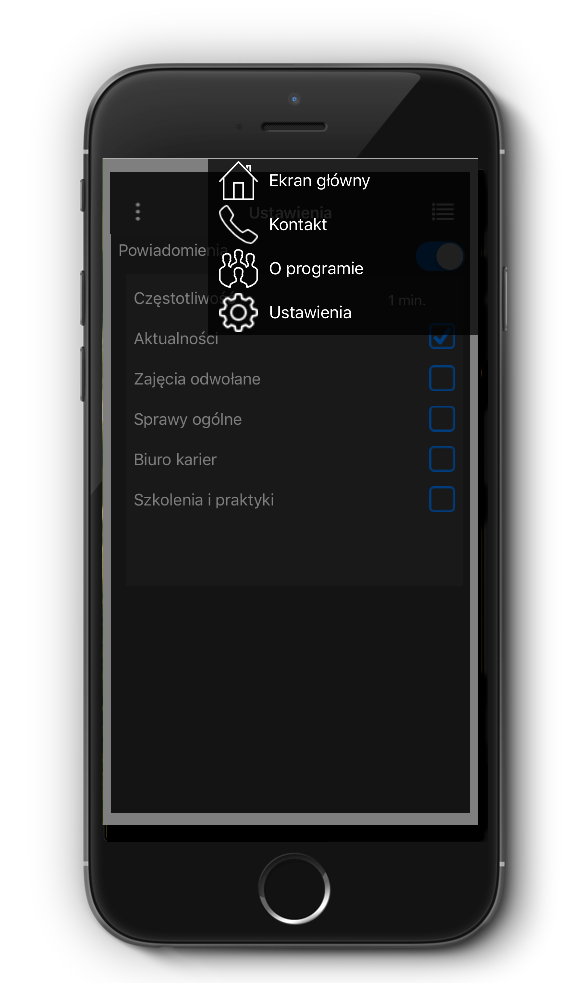
\includegraphics[width=.6\linewidth]{image/PraweIphone.png}
  \caption{Prawe menu}
  \label{fig:Prawe}
\end{subfigure}
\caption{Lewe oraz prawe menu aplikacji}
\label{fig:Menu}
\end{figure}
\begin{itemize}
\item \textbf{Ekran kontaku} -- Na ekranie widocznym na rysunku \ref{fig:Kontakt} wyświetlane są informacje potrzebne użytkownikowi przy kontakcie z wybranym instytutem. Oprócz adresu, który jest zwykłym tekstem reszta przycisków uruchamia przypisaną im odpowiednią reakcje. Po wybraniu przycisku z e-mailem uruchamiana jest systemowa skrzynka pocztowa użytkownika z nową wiadomością, także wystarczy wypełnić tylko temat i treść wiadomości. Przycisk z telefonem wybierze oraz zadzwoni na wyświetlony numer. Natomiast lokalizacja wyświetli nam dzięki pobranym współrzędnym z pliku konfiguracyjnego, instytut w systemowej aplikacji \textit{Mapy}. 
\end{itemize}
\newpage

\begin{itemize}

\item \textbf{Ekran o programie} -- Oprócz \textit{navigation bar}, które jest widoczne na każdym ekranie, widok składa się także z \textit{table view}. Na ekranie tym wyświetlani są twórcy, opiekun projektu, licencja oraz podziękowania. Wszystkie informacje pobierane są z pliku konfiguracyjnego i widoczne na rysunku  \ref{fig:Oprogramie}.
\item \textbf{Ekran ustawień} -- Rysunek \ref{fig:Ustawienia} przedstawia dostępne opcje do skonfigurowania przychodzących powiadomień. Główną opcją jest wyłączenie całkowite powiadomień co spowoduje ukrycie dodatkowych ustawień. Zawierają one częstotliwość z jaką aplikacja ma sprawdzać czy nowe informacje pojawiły się na stronie głównej instytutu oraz listę przycisków wyboru dostępnych kategorii.
\end{itemize}

\begin{figure}
\centering
\begin{minipage}{.5\textwidth}
  \centering
  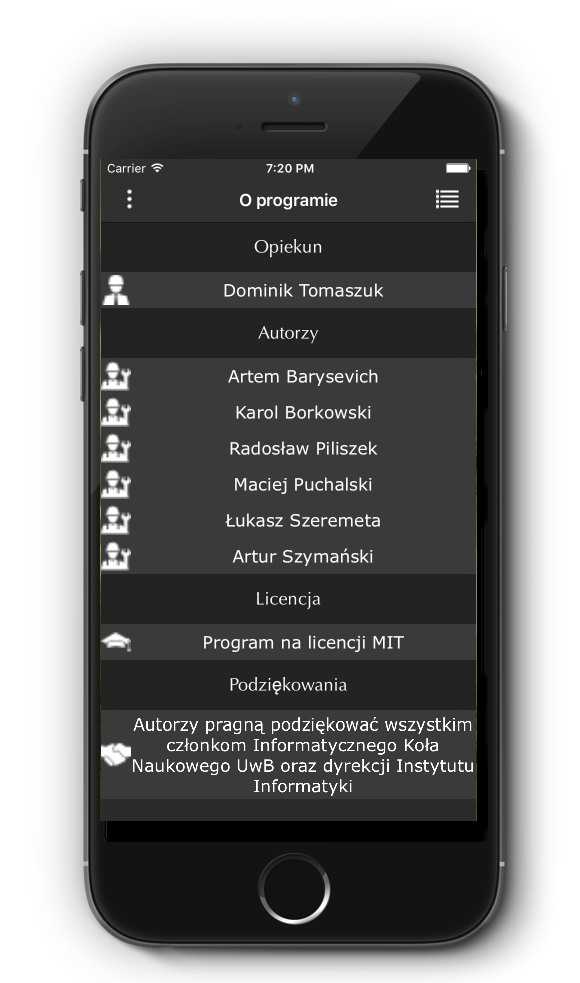
\includegraphics[width=.6\linewidth]{image/OprogramieIphone.png}
  \captionof{figure}{Ekran o programie}
  \label{fig:Oprogramie}
\end{minipage}%
\begin{minipage}{.5\textwidth}
  \centering
  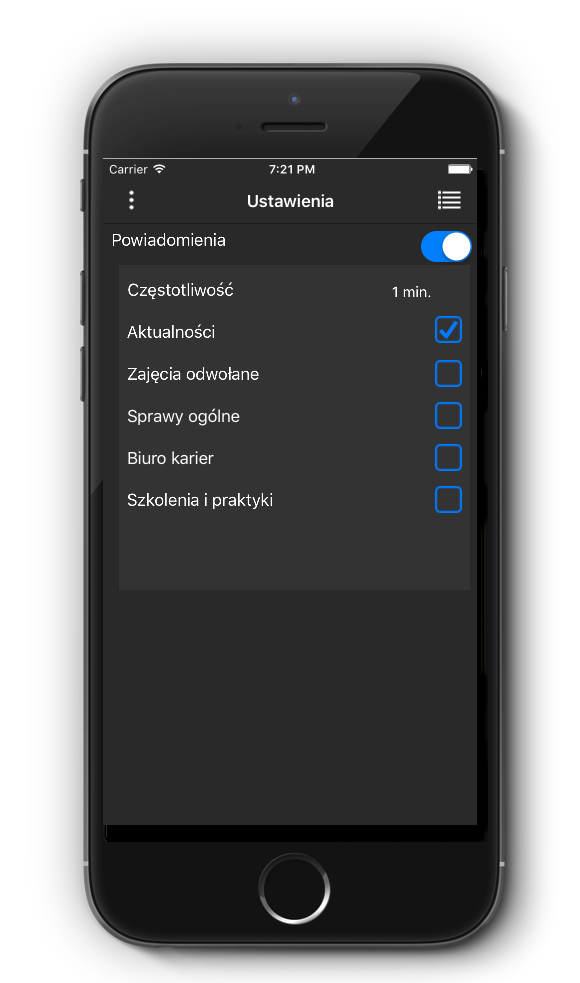
\includegraphics[width=.6\linewidth]{image/UstawieniaIphone.png}
  \captionof{figure}{Ekran ustawień}
  \label{fig:Ustawienia}
\end{minipage}
\end{figure}
\section{Architektura programu}
Całość projektu \textit{MobiUwB} pod względem architektury można podzielić na trzy zróżnicowane elementy, które razem ze sobą współgrają i komunikują poprzez przesył danych. Rysunek \ref{fig:architektura} przedstawia graficzny schemat architektury. Elementy te pełnią funkcje:
\begin{itemize}
\item \textbf{Element pierwszy} -- odpowiada za serwer, który przechowuje dane wyświetlane w elemencie drugim oraz trzecim. Dane przechowywane są w postaci plików konfiguracyjnych w formacie \textit{XML} jak i plików obejmujących informacje w formacie \textit{JSON} i \textit{XML}.
\item \textbf{Element drugi} -- jest to strona internetowa, która odpowiednio skonfigurowana pod urządzenia mobilne wyświetla informacje dostarczane z elementu pierwszego. Pokazywany jest w elemencie trzecim w przeglądarce internetowej i nie zależnie na jakim systemie operacyjnym jej wygląd pozostaję taki sam. 
\item \textbf{Element trzeci} -- jest aplikacją mobilną, którą głównym zadaniem jest wyświetlanie elementu drugiego w postaci strony \textit{WWW} w wbudowanej przeglądarce internetowej. Z pliku konfiguracyjnego elementu pierwszego czerpie informacje potrzebne do poprawnego działania notyfikacji oraz kontaktu z wybranym instytutem. Część ta jest głównym celem pracy licencjackiej.
\end{itemize}
\section{Użyte biblioteki}
\textit{CocoaPods}\footnote{\url{https://cocoapods.org} czas dostępu: 2016-06-01} jest oddzielną aplikacją pomagającą kierować w przejrzysty sposób bibliotekami użytymi w projekcie tworzonym w języku \textit{Objective-C} lub \textit{Swift}. Dzięki niej można w łatwy sposób wyszukać oraz zaimplementować biblioteki \textit{open-source}, tworząc bardziej scentralizowany ekosystem. Wybrane biblioteki umieszczane są w pliku tekstowym nazywanym \textit{Podfile} oraz za pomocą odpowiednich komend aplikacja pobiera, łączy oraz buduje ze sobą w obszarze roboczym programu \textit{Xcode}. Biblioteki użyte w projekcie:
\begin{itemize}
\item \textbf{SwiftyJSON}\footnote{\url{https://github.com/SwiftyJSON/SwiftyJSON} czas dostępu: 2016-06-01} -- biblioteka stworzona na licencji \textit{MIT}\footnote{MIT - typ licencji otwartego oprogramowania}, która ułatwia obsługę danych typu \textit{JSON} w \textit{Swift}. Użyta została do przetworzenia pliku konfiguracyjnego.
\item \textbf{SWXMLHash}\footnote{\url{https://github.com/drmohundro/SWXMLHash} czas dostępu: 2016-06-01} -- pozwala w relatywnie prosty sposób na parsowanie danych w formacie \textit{XML} na słownik tablic. Dzięki niej w łatwy sposób sparsowane zostały informacje o twórcach programu pobrane z pliku konfiguracyjnego \textit{XML}.
\end{itemize}
\newpage
\begin{itemize}
\item \textbf{SlideMenuControllerSwift}\footnote{\url{https://github.com/dekatotoro/SlideMenuControllerSwift} czas dostępu: 2016-06-01} -- biblioteka odpowiedzialna za prawe i lewe menu aplikacji, zaimplementowana oprócz podstawowych funkcjonalności zapewnia obsługę gestów oraz blokadę ekranu poza wysuwanym widokiem.
\item \textbf{Alamofire}\footnote{\url{https://github.com/Alamofire/Alamofire} czas dostępu: 2016-06-01} -- jest biblioteka obsługującą asynchronicznie połączenia sieciowe \textit{HTTP} w \textit{Swift}. Wykorzystuje do tego wbudowany \textit{framework Foundation} by zapewnić jak najszybsze możliwości sieciowe przy dogodnym interfejsie.
\end{itemize}

\begin{figure}[!th]
\centering
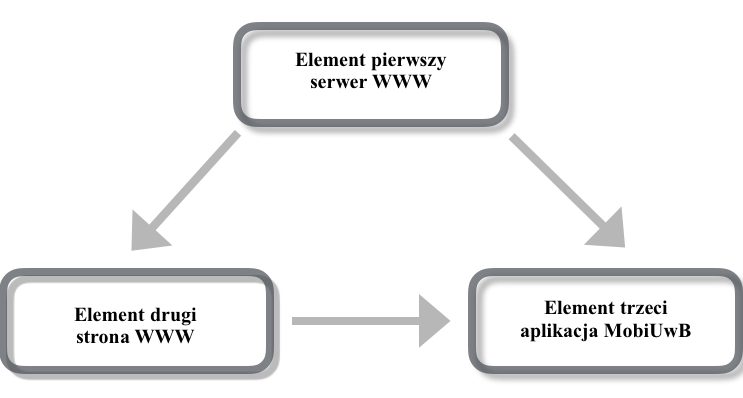
\includegraphics[scale=.5]{image/architektura.png}
\caption{Schemat architektury aplikacji}
\label{fig:architektura}
\end{figure}
%\section{Schematy Konfiguracji}
%
%\subsection{Schematy XML}
%
%\subsection{Schematy JSON}

\cleardoublepage
%\chapter*{Bibliografia}                                             
\addcontentsline{toc}{chapter}{Bibliografia} 
\bibliographystyle{plain}
\bibliography{myBib}
\end{document}